% Options for packages loaded elsewhere
\PassOptionsToPackage{unicode}{hyperref}
\PassOptionsToPackage{hyphens}{url}
\PassOptionsToPackage{dvipsnames,svgnames,x11names}{xcolor}
%
\documentclass[
  super,
  preprint,
  3p]{elsarticle}

\usepackage{amsmath,amssymb}
\usepackage{iftex}
\ifPDFTeX
  \usepackage[T1]{fontenc}
  \usepackage[utf8]{inputenc}
  \usepackage{textcomp} % provide euro and other symbols
\else % if luatex or xetex
  \usepackage{unicode-math}
  \defaultfontfeatures{Scale=MatchLowercase}
  \defaultfontfeatures[\rmfamily]{Ligatures=TeX,Scale=1}
\fi
\usepackage{lmodern}
\ifPDFTeX\else  
    % xetex/luatex font selection
\fi
% Use upquote if available, for straight quotes in verbatim environments
\IfFileExists{upquote.sty}{\usepackage{upquote}}{}
\IfFileExists{microtype.sty}{% use microtype if available
  \usepackage[]{microtype}
  \UseMicrotypeSet[protrusion]{basicmath} % disable protrusion for tt fonts
}{}
\makeatletter
\@ifundefined{KOMAClassName}{% if non-KOMA class
  \IfFileExists{parskip.sty}{%
    \usepackage{parskip}
  }{% else
    \setlength{\parindent}{0pt}
    \setlength{\parskip}{6pt plus 2pt minus 1pt}}
}{% if KOMA class
  \KOMAoptions{parskip=half}}
\makeatother
\usepackage{xcolor}
\setlength{\emergencystretch}{3em} % prevent overfull lines
\setcounter{secnumdepth}{5}
% Make \paragraph and \subparagraph free-standing
\ifx\paragraph\undefined\else
  \let\oldparagraph\paragraph
  \renewcommand{\paragraph}[1]{\oldparagraph{#1}\mbox{}}
\fi
\ifx\subparagraph\undefined\else
  \let\oldsubparagraph\subparagraph
  \renewcommand{\subparagraph}[1]{\oldsubparagraph{#1}\mbox{}}
\fi

\usepackage{color}
\usepackage{fancyvrb}
\newcommand{\VerbBar}{|}
\newcommand{\VERB}{\Verb[commandchars=\\\{\}]}
\DefineVerbatimEnvironment{Highlighting}{Verbatim}{commandchars=\\\{\}}
% Add ',fontsize=\small' for more characters per line
\usepackage{framed}
\definecolor{shadecolor}{RGB}{241,243,245}
\newenvironment{Shaded}{\begin{snugshade}}{\end{snugshade}}
\newcommand{\AlertTok}[1]{\textcolor[rgb]{0.68,0.00,0.00}{#1}}
\newcommand{\AnnotationTok}[1]{\textcolor[rgb]{0.37,0.37,0.37}{#1}}
\newcommand{\AttributeTok}[1]{\textcolor[rgb]{0.40,0.45,0.13}{#1}}
\newcommand{\BaseNTok}[1]{\textcolor[rgb]{0.68,0.00,0.00}{#1}}
\newcommand{\BuiltInTok}[1]{\textcolor[rgb]{0.00,0.23,0.31}{#1}}
\newcommand{\CharTok}[1]{\textcolor[rgb]{0.13,0.47,0.30}{#1}}
\newcommand{\CommentTok}[1]{\textcolor[rgb]{0.37,0.37,0.37}{#1}}
\newcommand{\CommentVarTok}[1]{\textcolor[rgb]{0.37,0.37,0.37}{\textit{#1}}}
\newcommand{\ConstantTok}[1]{\textcolor[rgb]{0.56,0.35,0.01}{#1}}
\newcommand{\ControlFlowTok}[1]{\textcolor[rgb]{0.00,0.23,0.31}{#1}}
\newcommand{\DataTypeTok}[1]{\textcolor[rgb]{0.68,0.00,0.00}{#1}}
\newcommand{\DecValTok}[1]{\textcolor[rgb]{0.68,0.00,0.00}{#1}}
\newcommand{\DocumentationTok}[1]{\textcolor[rgb]{0.37,0.37,0.37}{\textit{#1}}}
\newcommand{\ErrorTok}[1]{\textcolor[rgb]{0.68,0.00,0.00}{#1}}
\newcommand{\ExtensionTok}[1]{\textcolor[rgb]{0.00,0.23,0.31}{#1}}
\newcommand{\FloatTok}[1]{\textcolor[rgb]{0.68,0.00,0.00}{#1}}
\newcommand{\FunctionTok}[1]{\textcolor[rgb]{0.28,0.35,0.67}{#1}}
\newcommand{\ImportTok}[1]{\textcolor[rgb]{0.00,0.46,0.62}{#1}}
\newcommand{\InformationTok}[1]{\textcolor[rgb]{0.37,0.37,0.37}{#1}}
\newcommand{\KeywordTok}[1]{\textcolor[rgb]{0.00,0.23,0.31}{#1}}
\newcommand{\NormalTok}[1]{\textcolor[rgb]{0.00,0.23,0.31}{#1}}
\newcommand{\OperatorTok}[1]{\textcolor[rgb]{0.37,0.37,0.37}{#1}}
\newcommand{\OtherTok}[1]{\textcolor[rgb]{0.00,0.23,0.31}{#1}}
\newcommand{\PreprocessorTok}[1]{\textcolor[rgb]{0.68,0.00,0.00}{#1}}
\newcommand{\RegionMarkerTok}[1]{\textcolor[rgb]{0.00,0.23,0.31}{#1}}
\newcommand{\SpecialCharTok}[1]{\textcolor[rgb]{0.37,0.37,0.37}{#1}}
\newcommand{\SpecialStringTok}[1]{\textcolor[rgb]{0.13,0.47,0.30}{#1}}
\newcommand{\StringTok}[1]{\textcolor[rgb]{0.13,0.47,0.30}{#1}}
\newcommand{\VariableTok}[1]{\textcolor[rgb]{0.07,0.07,0.07}{#1}}
\newcommand{\VerbatimStringTok}[1]{\textcolor[rgb]{0.13,0.47,0.30}{#1}}
\newcommand{\WarningTok}[1]{\textcolor[rgb]{0.37,0.37,0.37}{\textit{#1}}}

\providecommand{\tightlist}{%
  \setlength{\itemsep}{0pt}\setlength{\parskip}{0pt}}\usepackage{longtable,booktabs,array}
\usepackage{calc} % for calculating minipage widths
% Correct order of tables after \paragraph or \subparagraph
\usepackage{etoolbox}
\makeatletter
\patchcmd\longtable{\par}{\if@noskipsec\mbox{}\fi\par}{}{}
\makeatother
% Allow footnotes in longtable head/foot
\IfFileExists{footnotehyper.sty}{\usepackage{footnotehyper}}{\usepackage{footnote}}
\makesavenoteenv{longtable}
\usepackage{graphicx}
\makeatletter
\def\maxwidth{\ifdim\Gin@nat@width>\linewidth\linewidth\else\Gin@nat@width\fi}
\def\maxheight{\ifdim\Gin@nat@height>\textheight\textheight\else\Gin@nat@height\fi}
\makeatother
% Scale images if necessary, so that they will not overflow the page
% margins by default, and it is still possible to overwrite the defaults
% using explicit options in \includegraphics[width, height, ...]{}
\setkeys{Gin}{width=\maxwidth,height=\maxheight,keepaspectratio}
% Set default figure placement to htbp
\makeatletter
\def\fps@figure{htbp}
\makeatother

\makeatletter
\makeatother
\makeatletter
\makeatother
\makeatletter
\@ifpackageloaded{caption}{}{\usepackage{caption}}
\AtBeginDocument{%
\ifdefined\contentsname
  \renewcommand*\contentsname{Table of contents}
\else
  \newcommand\contentsname{Table of contents}
\fi
\ifdefined\listfigurename
  \renewcommand*\listfigurename{List of Figures}
\else
  \newcommand\listfigurename{List of Figures}
\fi
\ifdefined\listtablename
  \renewcommand*\listtablename{List of Tables}
\else
  \newcommand\listtablename{List of Tables}
\fi
\ifdefined\figurename
  \renewcommand*\figurename{Figure}
\else
  \newcommand\figurename{Figure}
\fi
\ifdefined\tablename
  \renewcommand*\tablename{Table}
\else
  \newcommand\tablename{Table}
\fi
}
\@ifpackageloaded{float}{}{\usepackage{float}}
\floatstyle{ruled}
\@ifundefined{c@chapter}{\newfloat{codelisting}{h}{lop}}{\newfloat{codelisting}{h}{lop}[chapter]}
\floatname{codelisting}{Listing}
\newcommand*\listoflistings{\listof{codelisting}{List of Listings}}
\makeatother
\makeatletter
\@ifpackageloaded{caption}{}{\usepackage{caption}}
\@ifpackageloaded{subcaption}{}{\usepackage{subcaption}}
\makeatother
\makeatletter
\@ifpackageloaded{tcolorbox}{}{\usepackage[skins,breakable]{tcolorbox}}
\makeatother
\makeatletter
\@ifundefined{shadecolor}{\definecolor{shadecolor}{rgb}{.97, .97, .97}}
\makeatother
\makeatletter
\makeatother
\makeatletter
\makeatother
\journal{Journal Name}
\ifLuaTeX
  \usepackage{selnolig}  % disable illegal ligatures
\fi
\usepackage[]{natbib}
\bibliographystyle{elsarticle-num}
\IfFileExists{bookmark.sty}{\usepackage{bookmark}}{\usepackage{hyperref}}
\IfFileExists{xurl.sty}{\usepackage{xurl}}{} % add URL line breaks if available
\urlstyle{same} % disable monospaced font for URLs
\hypersetup{
  pdftitle={The Application of Machine Learning to Predict NFL Running Back Performance},
  pdfauthor={Giovanni Lunetta; Sam Lutzel},
  pdfkeywords={Machine Learning, Predictive Analytics, Sports
Analytics},
  colorlinks=true,
  linkcolor={blue},
  filecolor={Maroon},
  citecolor={Blue},
  urlcolor={Blue},
  pdfcreator={LaTeX via pandoc}}

\setlength{\parindent}{6pt}
\begin{document}

\begin{frontmatter}
\title{The Application of Machine Learning to Predict NFL Running Back
Performance \\\large{STATS-5405} }
\author[1]{Giovanni Lunetta%
\corref{cor1}%
}
 \ead{giovanni.lunetta@uconn.edu} 
\author[1]{Sam Lutzel%
\corref{cor1}%
}
 \ead{samuel.lutzel@uconn.edu} 

\affiliation[1]{organization={University of
Connecticut, Statistics},addressline={2075 Hillside
Road},city={Storrs},postcode={6269},postcodesep={}}

\cortext[cor1]{Corresponding author}


        
\begin{abstract}
This study employs an ensemble of machine learning techniques, including
Multiple Linear Regression (MLR), Generalized Linear Models (GLM), and
XGBoost to enhance predictive analytics in the National Football League
(NFL). The research focuses on one of the most critical aspects of
football offense - the running game. In order to predict the yards
gained by NFL running backs following a handoff, the study analyzes a
plethora of player tracking data from the 2017 to 2019 seasons. It
integrates a variety of factors such as player positions, orientation,
and the situational context of the game, including down, distance, and
field position. This multifaceted approach aims to yield highly accurate
models that can serve as valuable tools for coaching staffs to optimize
play-calling, manage player workloads, and enhance game planning. The
predictive insights derived from this research are intended to support
teams in deploying their running backs more effectively, leading to
potentially improved outcomes on the field. As the NFL continues to
evolve with a greater emphasis on analytics, this study seeks to
contribute significantly to the field of sports analytics by providing a
model that underscores the importance of the running game in a
predominantly pass-oriented league.
\end{abstract}





\begin{keyword}
    Machine Learning \sep Predictive Analytics \sep 
    Sports Analytics
\end{keyword}
\end{frontmatter}
    \ifdefined\Shaded\renewenvironment{Shaded}{\begin{tcolorbox}[boxrule=0pt, breakable, sharp corners, frame hidden, borderline west={3pt}{0pt}{shadecolor}, interior hidden, enhanced]}{\end{tcolorbox}}\fi

\hypertarget{introduction}{%
\section{Introduction}\label{introduction}}

\hypertarget{background-of-the-national-football-league}{%
\subsection{Background of the National Football
League}\label{background-of-the-national-football-league}}

The National Football League (NFL) is the most popular professional
sports league in the United States, with an estimated 187 million fans.
The league consists of 32 teams divided into two conferences, the
American Football Conference (AFC) and the National Football Conference
(NFC). Each conference is further divided into four divisions, with four
teams in each division. The NFL season consists of 17 weeks, with each
team playing 16 games and having one bye week. The regular season is
followed by a 12-team playoff, with the winner of each conference
advancing to the Super Bowl, the league's championship game.

The NFL game strategy primarily consists of two ways to advance the
football down the field: running and passing. Running the ball is
defined as a play in which the quarterback gives the ball to another
player that is located behind them (a handoff or a small toss). The
player then attempts to run the ball down the field as far as possible
before being tackled to the ground. Passing the ball is defined as a
play in which the quarterback throws the ball to another player down the
field. The player then attempts to catch the ball and advance it down
the field as far as possible before being tackled to the ground. The
goal of each team is to score as many points as possible by advancing
the ball down the field and into the end zone or by kicking the ball
through the field goal posts. The team with the most points at the end
of the game wins.

\hypertarget{motivation}{%
\subsection{Motivation}\label{motivation}}

The primary goal of this research is to develop cutting-edge predictive
models capable of accurately estimating the yards a running back will
gain after a handoff during NFL games. This objective is pivotal for
formulating advanced offensive strategies and refining player
evaluations. The running play is a fundamental aspect of the game that
can dictate the tempo, control the clock, and establish physical
dominance.

The motivation behind this study stems from the transformative impact
that data analytics has had on sports, particularly in the NFL, where
the fusion of technology and sports science has begun to redefine how
the game is played and understood. In an era where marginal gains are
increasingly sought after, the ability to predict the outcome of running
plays with high precision can provide teams with a significant
competitive advantage. It enables coaches to make informed decisions
regarding play selection, player rotations, and game management,
especially in critical moments of a match. Additionally, the insights
from this study can empower front offices in their scouting and drafting
processes by quantifying the expected value a running back adds to their
team. Furthermore, there is also a tremendous opportunity to leverage
these predictive models on the defensive end of the ball, allowing teams
to better anticipate and defend against running plays. With better
insights into the opponents running game, defenses can adjust their
schemes and personnel to counter the opposing team's offensive strategy,
such as by stacking the box or blitzing the quarterback. In addition to
the benefits performance analytics provides to the teams, it also helps
fans select better fantasy football teams and make more informed betting
decisions. This leads to a more engaging and enjoyable experience for
the fans, which is critical for the long-term success of the league.

Ultimately, the true beauty of this research lies in its ability to
bridge the gap between complex player tracking data and practical
on-field strategies. In specific, it's about enhancing the very essence
of the game and enriching the broader discourse on sports performance
analytics. By pioneering research in this domain, this study is set to
propel the analytical capabilities of NFL teams to new heights,
providing them with tools that were once considered unimaginable.
Ultimately, it contributes to the ongoing evolution of the sport itself,
marking a pivotal moment in the history of football and the broader
world of sports analytics.

\hypertarget{methods}{%
\section{Methods}\label{methods}}

\hypertarget{data-cleaning-and-preprocessing}{%
\subsection{Data Cleaning and
Preprocessing}\label{data-cleaning-and-preprocessing}}

Data cleaning and preprocessing are critical to ensuring the quality and
integrity of machine learning models. The cleaned dataset was obtained
by addressing any inconsistencies and handling missing data through
imputation techniques. Preprocessing steps included encoding categorical
variables using one-hot encoding or label encoding methods and scaling
and normalizing numerical variables to ensure they are on comparable
scales.

To begin, several variables were removed in order to simulate the
beginning of each play. For instance, the dataset include the speed,
acceleration, direction, and distance traveled of each player on the
field at the beginning of each play. However, this information is not
available to the coaching staff prior to the snap of the ball.
Therefore, these variables were removed from the datset. Furthermore,
some variables may introduce multicollinearity issues since they
represent the same information. For instance, the dataset includes the
name and id of each player on the field. However, these variables are
highly correlated with each other. Therefore, only one of these
variables was kept in the dataset.

When the dataset was first obtained, each row represented a single
player on the field. However, the goal of this study is to predict the
yards gained after a handoff for each play. Therefore, every 22 rows had
to be merged into one row (11 players on each side). During this
process, any duplicated information/columns were dropped from the
dataset. One example of this is the weather during the play. When all 22
rows are merged, it included the weather 22 times, even though weather
is only needed once.

In addition to the attempt at removing unnecessary variables and
proactively removing potenital multicollienarity issues, variables such
as weather, wind speed, and wind direction had multiple levels, some of
which represented the same data. For instance, ``rainy'' and ``showers''
were considered the same weather type. There were multiple instances of
relationships between inputs on the same variable that existed similar
to the example above. Due to this, these weather types were grouped into
one category - ``rain.'' This helps to drastically reduce the complexity
of the dataset. These variables were also converted to factors for the
modeling process.

Variables such as offense personnel had to be converted to dummy
variables. The input for each dummy variable was either 0 or 1 depending
on whether or not the offense had that personnel on the field. For
instance, if the offense had 2 running backs on the field, the input for
the ``RB'' dummy variable would be 2. The input for the ``WR'' dummy
variable would be 0 since there were no wide receivers on the field.
This process was repeated for all personnel types.

One additional step that was taken was the randomization of all plays
within the dataset. The reason for this randomization is to ensure that
each row (play of a game) is independent of one another. Furthermore,
the dataset only contains running plays. Therefore, passing plays that
occured between the running plays were removed. In other words, all
plays are not dependent on the previous outcome. In all, the
randomization of the dataset in conjunction with the removal of passing
plays ensures that each row is independent of one another.

\hypertarget{data-exploration}{%
\subsection{Data Exploration}\label{data-exploration}}

Prior to the development of the predictive models, a comprehensive
exploratory data analysis (EDA) was conducted to understand the
underlying structure and characteristics of the data. This step involved
visualizing the distribution of key variables, identifying patterns and
outliers, and exploring correlations and interactions between
predictors. Data visualization, through techniques like scatter plots,
histograms, and heatmaps, can offer an intuitive understanding of data
distributions, correlations, and potential clusters within the dataset.
EDA-informed feature selection and engineering strategies highlighted
potential predictors that are most informative of yards gained after a
handoff.

\hypertarget{feature-engineering}{%
\subsection{Feature Engineering}\label{feature-engineering}}

During preprocessing, we will also undertake feature engineering to
create new variables that may have a stronger relationship with the
target variable. This could include interaction terms that capture the
combined effect of two predictors, polynomial features for capturing
non-linear relationships, and domain-specific features that encapsulate
strategic elements of the game.

\hypertarget{model-development-and-evaluation}{%
\subsection{Model Development and
Evaluation}\label{model-development-and-evaluation}}

With a clean and prepared dataset, we will then proceed to develop our
MLR, GLM, and XGBoost models.

\hypertarget{multiple-linear-regression-mlr}{%
\subsection{Multiple Linear Regression
(MLR)}\label{multiple-linear-regression-mlr}}

Multiple linear regression models predict a continuous repsonse variable
using a linear combination of predictors. For our baseline MLR model, we
will use the ordinary least squares (OLS) method to estimate the
coefficients of our predictor variables. The model is specified as:

\(Y_i = \beta_0 + \beta_1X_{i1} + \beta_2X_{i2} + \ldots + \beta_jX_{ij} + \epsilon_i\)

where \(Y_i\) represents the yards gained after the handoff for the
\(i^{th}\) observation, \(X_{ij}\) is the \(i^{th}\) observation on the
\(j^{th}\) predictor variable (where \(j = 1, ..., p\)),~\(\beta_j\) is
the \(j^{th}\) coefficient to be estimated corresponding to the proper
\(X_{ij}\) variable, and \(\epsilon_i\) is the error term. The
\(j^{th}\) coefficient, \(\beta_j\), represents the change in the
response variable for a unit change in the \(X_{ij}\) predictor
variable, while holding all other predictors constant.

The ordinary least squares (OLS) method will be deployed to minimize the
sum of the squared differences between the observed and predicted
values. The optimization problem can be represented as minimizing the
sum of errors squared:

\[
\Sigma_{i=0}^n \epsilon_i^2 = \Sigma_{i=0}^n (Y_i - \hat{Y}_i)^2 = \Sigma_{i=0}^n (Y_i - \beta_0 - \beta_1X_{i1} - \ldots - \beta_jX_{ij})^2
\]

Here, \(\Sigma_{i=0}^n \epsilon_i^2\) represents the sum of the squared
residuals, which we aim to minimize. The variable \(\hat{Y}_i\)
represents the predicted outcome of the model for the \(i^{th}\)
observation. This approach assumes that the relationship between the
independent variables and the dependent variable is linear. To ensure
the robustness of our model, we will conduct a series of diagnostic
tests:

\begin{enumerate}
\def\labelenumi{\arabic{enumi}.}
\tightlist
\item
  Linearity: We will use scatter plots and residual plots to verify that
  the relationship between the predictors and the response is linear.
\item
  Homoscedasticity: We will inspect the residuals to confirm constant
  variance across all levels of the independent variables. This can be
  assessed visually using a residual vs.~fitted values plot.
\item
  Independence: The Durbin-Watson test will help in detecting the
  presence of autocorrelation in the residuals, which should not be
  present in the data.
\item
  Normality of Residuals: Normality will be checked using Q-Q plots and
  statistical tests like the Shapiro-Wilk test.
\end{enumerate}

If any assumptions are violated, we may consider transformations of
variables or the use of robust regression techniques.

\hypertarget{generalized-linear-models-glm}{%
\subsection{Generalized Linear Models
(GLM)}\label{generalized-linear-models-glm}}

GLMs extend the linear model framework to allow for response variables
that have error distribution models other than a normal distribution.
They are particularly useful when dealing with non-normal response
variables, such as count data or binary outcomes. In its general form, a
GLM consists of three elements:

\begin{enumerate}
\def\labelenumi{\arabic{enumi}.}
\tightlist
\item
  Random Component: Specifies the probability distribution of the
  response variable \(Y\), such as normal, binomial, Poisson, or
  exponential.
\item
  Systematic Component: A linear predictor \(\eta = X\beta\).
\item
  Link Function: A function \(g\) that relates the mean of the response
  variable \(E(Y)\) to the linear predictor \(\eta\).
\end{enumerate}

The choice of link function is crucial and is typically selected based
on the nature of the distribution of the response variable. For
instance, a logit link function is used for a binomial distribution, and
a log link function is often used for a Poisson distribution.

The likelihood function for a GLM can be written as:

\[
L(\beta) = \prod_{i=1}^{n} f(y_i; \theta_i, \phi)
\]

where \(f(y_i; \theta_i, \phi)\) is the probability function for the
\(i\)-th observation, \(\theta_i\) is the parameter of interest (e.g.,
mean), and \(\phi\) is the dispersion parameter. The goal is to find the
values of \(\beta\) that maximize this likelihood function.

\hypertarget{xgboost}{%
\subsection{XGBoost}\label{xgboost}}

XGBoost stands for eXtreme Gradient Boosting and is a
decision-tree-based ensemble Machine Learning algorithm that uses a
gradient boosting framework. It is a powerful technique that can handle
a variety of regression and classification problems. For regression, it
can be configured to optimize for different loss functions; the most
common for regression being the squared error loss:

\[
L(\theta) = \sum_{i=1}^{n}(y_i - \hat{y}_i)^2
\]

where \(y_i\) are the observed values, and \(\hat{y}_i\) are the
predicted values.

In XGBoost, each new tree is built to correct the errors made by the
previous ones. The algorithm combines weak predictive models to form a
strong predictor. The model's complexity is controlled by the
regularization term \(\Omega(\theta)\) which is a function of the tree
structure and the number of leaves. The overall objective function to be
minimized is:

\[
\text{Obj}(\theta) = L(\theta) + \lambda \sum_{k}(w_k^2) + \gamma T
\]

where \(w_k\) represents the leaf weights of the trees, \(T\) is the
number of leaves, \(\lambda\) is the L2 regularization term on the
weights, and \(\gamma\) is the complexity control on the number of
leaves. For regression tasks, we can also utilize the quantile loss
which is particularly useful for prediction intervals:

\[
L_{\tau}(\theta) = \sum_{i=1}^{n} \left[ \tau (y_i - \hat{y}_i) \mathbb{1}_{y_i \geq \hat{y}_i} + (1 - \tau) (\hat{y}_i - y_i) \mathbb{1}_{y_i < \hat{y}_i} \right]
\]

Here, 1 is an indicator function, and \(\tau\) is the quantile of
interest, allowing us to model different parts of the conditional
distribution of the response variable.

XGBoost also provides a feature importance score, which is a metric that
quantifies the contribution of each feature to the model's predictive
power. This is done by measuring the impact on the model's accuracy each
time a feature is used to split the data across all trees.

\hypertarget{model-performance-metrics}{%
\subsection{Model Performance Metrics}\label{model-performance-metrics}}

For MLR and GLM, the model's performance will be evaluated using metrics
such as the Mean Squared Error (MSE) and the Mean Absolute Error (MAE).
For the XGBoost model, along with MSE and MAE, we will assess
performance using additional metrics like the R-squared for regression
tasks and feature importance scores to understand which variables are
most predictive.

\hypertarget{model-interpretation-and-application}{%
\subsection{Model Interpretation and
Application}\label{model-interpretation-and-application}}

The final step will be to interpret the models in the context of NFL
games. This will involve translating the statistical outputs into
actionable insights for coaches and team strategists, providing
recommendations on how to leverage the results for competitive advantage
in play-calling and player evaluation.

\hypertarget{software-and-tools}{%
\subsection{Software and Tools}\label{software-and-tools}}

All analyses will be conducted in R, a statistical computing language
that provides a wide array of packages for machine learning and data
analysis. For MLR and GLM, we will utilize the \texttt{stats} package
that comes with the R base installation. For our XGBoost model, we will
use the \texttt{xgboost} package, which is specifically designed for
speed and performance. Data manipulation and cleansing will be managed
with packages like \texttt{dplyr} and \texttt{tidyr}, while
\texttt{ggplot2} will be employed for data visualization to facilitate
understanding and interpretation of the data and model outputs. For
feature engineering and preprocessing, we will take advantage of
\texttt{caret} or \texttt{recipes}. Hyperparameter tuning can be
optimized using the \texttt{tune} package, and for cross-validation, the
\texttt{rsample} package will be employed. The \texttt{broom} and
\texttt{modelr} packages will be useful for tidying model outputs and
working with models in a pipeline, respectively. This suite of packages
will enable a comprehensive workflow within R for developing,
evaluating, and interpreting the predictive models.

\hypertarget{model-development}{%
\subsection{Model Development}\label{model-development}}

To commence our analytical journey, we initiate with Multiple Linear
Regression (MLR) as our foundational modeling technique. This approach
is not just a stepping stone, but a critical phase in our analysis,
offering valuable insights into the relationships between various
features of the game and the yards gained. MLR helps discern the linear
associations and relative importance of different variables, setting the
stage for more complex modeling. Subsequent to this exploratory
analysis, we transition to XGBoost, an advanced machine learning
technique renowned for its predictive power and efficiency. XGBoost, a
gradient boosting framework, is chosen for its ability to handle the
dataset's complexity, non-linear relationships, and interactions among
variables more adeptly. This shift from MLR to XGBoost embodies our
methodological progression, from understanding the foundational
relationships in our data to harnessing advanced computational
techniques for more accurate and robust predictions in the dynamic and
unpredictable context of NFL games.

\hypertarget{multiple-linear-regression-model}{%
\section{Multiple Linear Regression
Model}\label{multiple-linear-regression-model}}

First, lets start by importing the completely clean and ready to use
dataset. This dataset was the result of procedures outlined in the data
cleaning and preprocessing section.

\begin{Shaded}
\begin{Highlighting}[]
\CommentTok{\# Import the dataset}
\NormalTok{football\_data }\OtherTok{\textless{}{-}} \FunctionTok{read.csv}\NormalTok{(}\StringTok{"/Users/samlutz10/Desktop/STAT5405/Final Project/train\_ready.csv"}\NormalTok{)}

\FunctionTok{str}\NormalTok{(football\_data)}
\end{Highlighting}
\end{Shaded}

\begin{verbatim}
'data.frame':   31007 obs. of  21 variables:
 $ Quarter          : int  2 2 4 2 2 1 2 4 4 4 ...
 $ Down             : int  1 1 1 2 1 1 1 1 1 1 ...
 $ Distance         : int  10 10 10 10 10 10 10 10 10 10 ...
 $ OffenseFormation : chr  "SINGLEBACK" "I_FORM" "I_FORM" "SINGLEBACK" ...
 $ RB               : int  2 2 2 1 1 1 1 1 2 1 ...
 $ TE               : int  1 1 2 1 1 2 1 1 1 1 ...
 $ WR               : int  2 2 1 3 3 2 3 3 1 3 ...
 $ DefendersInTheBox: int  8 7 8 6 7 8 6 7 7 7 ...
 $ Yards            : int  1 12 3 -2 14 4 3 7 7 3 ...
 $ Week             : int  3 9 14 2 2 2 17 11 17 3 ...
 $ GameWeather      : chr  "clear" "overcast" "clear" "clear" ...
 $ Temperature      : int  84 77 39 81 79 79 19 68 71 68 ...
 $ Humidity         : int  25 62 55 45 48 48 36 54 66 42 ...
 $ WindSpeed        : num  5 16 11 5 5 5 12 4 9 13 ...
 $ WindDirection    : chr  "west" "south east" "none" "east" ...
 $ GameHour         : int  15 9 3 3 13 12 2 6 15 12 ...
 $ DL               : int  4 3 4 4 2 4 2 4 4 4 ...
 $ LB               : int  3 4 3 2 4 3 4 2 3 2 ...
 $ BL               : int  4 4 4 5 5 4 5 5 4 5 ...
 $ YardsFromOwnGoal : int  40 84 79 21 86 25 49 25 65 54 ...
 $ ScoreDelta       : int  -7 0 -13 -11 0 7 -11 41 -16 -8 ...
\end{verbatim}

Since we are only focused on the most common plays and not breakout
runs, we will remove any data of 10 yards or more. This is due to the
fact that plays resulting in 10 yards are considered to be just as
successful are play resulting in more than 10 yards. In addition, any
plays resulting in 0 or negative yards will be removed. This is due to
the fact that these plays are considered to be unsuccessful.

\begin{Shaded}
\begin{Highlighting}[]
\CommentTok{\# Remove any rows whose yards column is greater than 30}
\NormalTok{football\_data }\OtherTok{\textless{}{-}}\NormalTok{ football\_data[football\_data}\SpecialCharTok{$}\NormalTok{Yards }\SpecialCharTok{\textless{}=} \DecValTok{10} \SpecialCharTok{\&}\NormalTok{ football\_data}\SpecialCharTok{$}\NormalTok{Yards }\SpecialCharTok{\textgreater{}} \DecValTok{0}\NormalTok{, ]}
\end{Highlighting}
\end{Shaded}

Lets now look at the histogram of Yards to get a better understanding of
the distribution of the response variable.

\begin{Shaded}
\begin{Highlighting}[]
\CommentTok{\# Histogram of Yards}
\FunctionTok{hist}\NormalTok{(football\_data}\SpecialCharTok{$}\NormalTok{Yards, }\AttributeTok{main =} \StringTok{"Histogram of Yards"}\NormalTok{, }\AttributeTok{xlab =} \StringTok{"Yards"}\NormalTok{, }\AttributeTok{ylab =} \StringTok{"Frequency"}\NormalTok{, }\AttributeTok{col =} \StringTok{"blue"}\NormalTok{)}
\end{Highlighting}
\end{Shaded}

\begin{figure}[H]

{\centering \includegraphics{project_report_files/figure-pdf/unnamed-chunk-3-1.pdf}

}

\end{figure}

Based on the histogram above, it is apparent that the number of yards is
skewed to the right. In order to address this issue, the Box-Cox
transformation will be utilized. This will help to normalize the
distribution of the response variable. The Box-Cox transformation can
transform non-normal data into normal data.

\begin{Shaded}
\begin{Highlighting}[]
\FunctionTok{library}\NormalTok{(MASS)}
\NormalTok{lambda\_null }\OtherTok{\textless{}{-}} \FunctionTok{boxcox}\NormalTok{(}\FunctionTok{lm}\NormalTok{(Yards }\SpecialCharTok{\textasciitilde{}} \DecValTok{1}\NormalTok{, }\AttributeTok{data =}\NormalTok{ football\_data))}
\end{Highlighting}
\end{Shaded}

\begin{figure}[H]

{\centering \includegraphics{project_report_files/figure-pdf/unnamed-chunk-4-1.pdf}

}

\end{figure}

The best lambda value for the Box-Cox tranformation is as follows:

\begin{Shaded}
\begin{Highlighting}[]
\NormalTok{lambda\_null}\SpecialCharTok{$}\NormalTok{x[}\FunctionTok{which.max}\NormalTok{(lambda\_null}\SpecialCharTok{$}\NormalTok{y)]}
\end{Highlighting}
\end{Shaded}

\begin{verbatim}
[1] 0.2222222
\end{verbatim}

Now the Box-Cox tranformation will be applied to the variable Yards with
the best lambda value.

\begin{Shaded}
\begin{Highlighting}[]
\NormalTok{lm\_model\_null }\OtherTok{\textless{}{-}} \FunctionTok{lm}\NormalTok{((Yards}\SpecialCharTok{\^{}}\NormalTok{(lambda\_null}\SpecialCharTok{$}\NormalTok{x[}\FunctionTok{which.max}\NormalTok{(lambda\_null}\SpecialCharTok{$}\NormalTok{y)])) }\SpecialCharTok{\textasciitilde{}} \DecValTok{1}\NormalTok{, }\AttributeTok{data =}\NormalTok{ football\_data)}
\FunctionTok{summary}\NormalTok{(lm\_model\_null)}
\end{Highlighting}
\end{Shaded}

\begin{verbatim}

Call:
lm(formula = (Yards^(lambda_null$x[which.max(lambda_null$y)])) ~ 
    1, data = football_data)

Residuals:
     Min       1Q   Median       3Q      Max 
-0.30438 -0.13785 -0.02786  0.12559  0.36373 

Coefficients:
            Estimate Std. Error t value Pr(>|t|)    
(Intercept)   1.3044     0.0013    1003   <2e-16 ***
---
Signif. codes:  0 '***' 0.001 '**' 0.01 '*' 0.05 '.' 0.1 ' ' 1

Residual standard error: 0.1924 on 21900 degrees of freedom
\end{verbatim}

Now the full model using all of the predictors will be created. In this
full model, there will be 0 interactions between the predictors. The
same process using the Box-Cox transformation will be used to normalize
the distribution of the response variable.

\begin{Shaded}
\begin{Highlighting}[]
\NormalTok{lambda\_full }\OtherTok{\textless{}{-}} \FunctionTok{boxcox}\NormalTok{(}\FunctionTok{lm}\NormalTok{(Yards }\SpecialCharTok{\textasciitilde{}}\NormalTok{ ., }\AttributeTok{data =}\NormalTok{ football\_data))}
\end{Highlighting}
\end{Shaded}

\begin{figure}[H]

{\centering 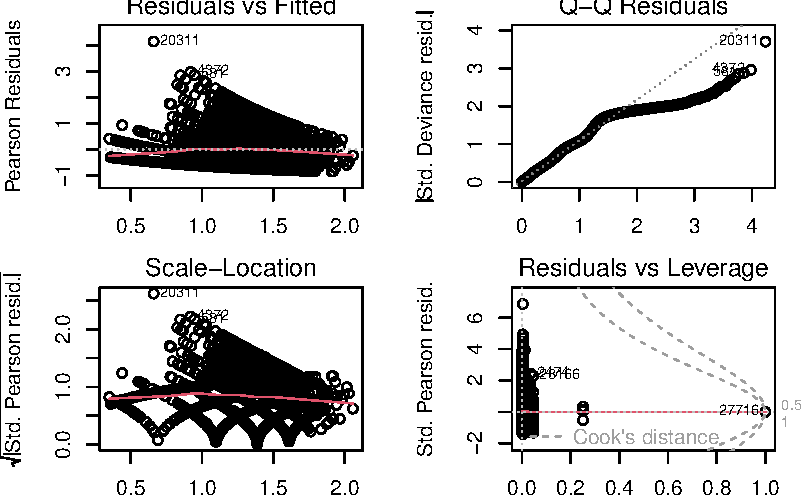
\includegraphics{project_report_files/figure-pdf/unnamed-chunk-7-1.pdf}

}

\end{figure}

The best lambda value for the Box-Cox tranformation is as follows:

\begin{Shaded}
\begin{Highlighting}[]
\NormalTok{lambda\_full}\SpecialCharTok{$}\NormalTok{x[}\FunctionTok{which.max}\NormalTok{(lambda\_full}\SpecialCharTok{$}\NormalTok{y)]}
\end{Highlighting}
\end{Shaded}

\begin{verbatim}
[1] 0.2222222
\end{verbatim}

Now the Box-Cox tranformation will be applied to the variable Yards with
the best lambda value.

\begin{Shaded}
\begin{Highlighting}[]
\NormalTok{lm\_model\_full }\OtherTok{\textless{}{-}} \FunctionTok{lm}\NormalTok{((Yards}\SpecialCharTok{\^{}}\NormalTok{(lambda\_full}\SpecialCharTok{$}\NormalTok{x[}\FunctionTok{which.max}\NormalTok{(lambda\_full}\SpecialCharTok{$}\NormalTok{y)])) }\SpecialCharTok{\textasciitilde{}}\NormalTok{ ., }\AttributeTok{data =}\NormalTok{ football\_data)}
\FunctionTok{summary}\NormalTok{(lm\_model\_full)}
\end{Highlighting}
\end{Shaded}

\begin{verbatim}

Call:
lm(formula = (Yards^(lambda_full$x[which.max(lambda_full$y)])) ~ 
    ., data = football_data)

Residuals:
     Min       1Q   Median       3Q      Max 
-0.47321 -0.13673  0.00441  0.13919  0.47383 

Coefficients:
                             Estimate Std. Error t value Pr(>|t|)    
(Intercept)                 1.538e+00  4.252e-01   3.617 0.000299 ***
Quarter                     1.967e-04  1.126e-03   0.175 0.861252    
Down                        4.977e-03  2.256e-03   2.206 0.027365 *  
Distance                    3.810e-03  4.147e-04   9.186  < 2e-16 ***
OffenseFormationEMPTY       2.472e-02  1.924e-01   0.129 0.897743    
OffenseFormationI_FORM     -1.687e-02  1.882e-01  -0.090 0.928585    
OffenseFormationJUMBO      -1.033e-01  1.885e-01  -0.548 0.583848    
OffenseFormationPISTOL     -1.455e-02  1.883e-01  -0.077 0.938427    
OffenseFormationSHOTGUN    -2.890e-02  1.882e-01  -0.154 0.877950    
OffenseFormationSINGLEBACK -1.774e-02  1.882e-01  -0.094 0.924890    
OffenseFormationUNKNOWN    -4.250e-02  2.104e-01  -0.202 0.839923    
OffenseFormationWILDCAT     9.191e-04  1.898e-01   0.005 0.996136    
RB                         -2.884e-03  5.899e-03  -0.489 0.624916    
TE                         -6.842e-04  4.914e-03  -0.139 0.889284    
WR                         -6.221e-03  5.009e-03  -1.242 0.214249    
DefendersInTheBox          -2.753e-02  1.957e-03 -14.068  < 2e-16 ***
Week                       -2.674e-04  3.456e-04  -0.774 0.439106    
GameWeathernone             7.031e-03  4.258e-03   1.651 0.098726 .  
GameWeatherovercast        -8.048e-04  3.130e-03  -0.257 0.797075    
GameWeatherrain            -5.022e-03  6.343e-03  -0.792 0.428550    
GameWeathersnow            -1.267e-02  1.845e-02  -0.687 0.492132    
Temperature                -3.322e-04  1.013e-04  -3.279 0.001045 ** 
Humidity                   -2.549e-05  6.333e-05  -0.402 0.687361    
WindSpeed                  -5.975e-06  3.116e-04  -0.019 0.984703    
WindDirectionnone          -1.113e-02  8.175e-03  -1.361 0.173435    
WindDirectionnorth         -5.339e-03  9.551e-03  -0.559 0.576202    
WindDirectionnorth east    -8.907e-03  8.227e-03  -1.083 0.278988    
WindDirectionnorth west    -5.889e-03  8.309e-03  -0.709 0.478510    
WindDirectionsouth         -8.759e-03  9.043e-03  -0.969 0.332759    
WindDirectionsouth east    -5.197e-03  8.566e-03  -0.607 0.544061    
WindDirectionsouth west    -6.548e-03  8.069e-03  -0.811 0.417105    
WindDirectionwest          -5.602e-03  9.642e-03  -0.581 0.561220    
GameHour                    5.532e-04  2.930e-04   1.888 0.059064 .  
DL                         -2.472e-03  3.461e-02  -0.071 0.943047    
LB                         -3.311e-03  3.469e-02  -0.095 0.923948    
BL                          4.935e-03  3.469e-02   0.142 0.886864    
YardsFromOwnGoal           -4.004e-04  5.338e-05  -7.500 6.65e-14 ***
ScoreDelta                 -2.002e-04  1.209e-04  -1.656 0.097793 .  
---
Signif. codes:  0 '***' 0.001 '**' 0.01 '*' 0.05 '.' 0.1 ' ' 1

Residual standard error: 0.1881 on 21584 degrees of freedom
  (279 observations deleted due to missingness)
Multiple R-squared:  0.04689,   Adjusted R-squared:  0.04525 
F-statistic:  28.7 on 37 and 21584 DF,  p-value: < 2.2e-16
\end{verbatim}

Based on the results of the full model, the model shows which predictors
are statistically significant. The most significant predictors are
Distance, DefendersInTheBox, and YardsFromOwnGoal. Creating scatter
plots of the response variable versus each of these predictors will help
to gain a better understanding of how these variables affect the
predicted yards.

\begin{Shaded}
\begin{Highlighting}[]
\CommentTok{\# Scatter plot of yards vs. Distance}
\FunctionTok{plot}\NormalTok{(football\_data}\SpecialCharTok{$}\NormalTok{Yards, football\_data}\SpecialCharTok{$}\NormalTok{Distance, }\AttributeTok{main =} \StringTok{"Yards vs. Distance"}\NormalTok{, }\AttributeTok{xlab =} \StringTok{"Yards"}\NormalTok{, }\AttributeTok{ylab =} \StringTok{"Distance"}\NormalTok{, }\AttributeTok{pch =} \DecValTok{19}\NormalTok{)}
\end{Highlighting}
\end{Shaded}

\begin{figure}[H]

{\centering 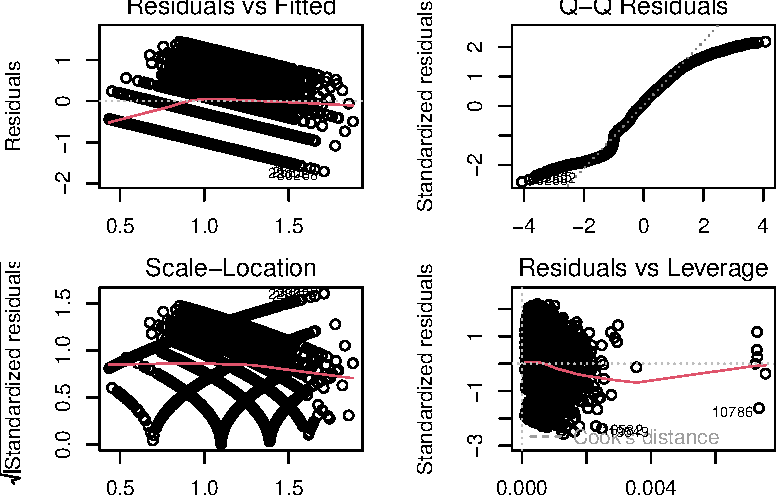
\includegraphics{project_report_files/figure-pdf/unnamed-chunk-10-1.pdf}

}

\end{figure}

Looking at this scatter plot of Yards vs Distance, there appears to only
be a sinusoial relationship between the two variables. Therefore, when a
reduced model is created, a sine function will be used to model the
relationship between the two variables.

\begin{Shaded}
\begin{Highlighting}[]
\CommentTok{\# Scatter plot of yards vs. Defenders In The Box}
\FunctionTok{plot}\NormalTok{(football\_data}\SpecialCharTok{$}\NormalTok{Yards, football\_data}\SpecialCharTok{$}\NormalTok{DefendersInTheBox, }\AttributeTok{main =} \StringTok{"Yards vs. Defenders In The Box"}\NormalTok{, }\AttributeTok{xlab =} \StringTok{"Yards"}\NormalTok{, }\AttributeTok{ylab =} \StringTok{"Defenders In The Box"}\NormalTok{, }\AttributeTok{pch =} \DecValTok{19}\NormalTok{)}
\end{Highlighting}
\end{Shaded}

\begin{figure}[H]

{\centering 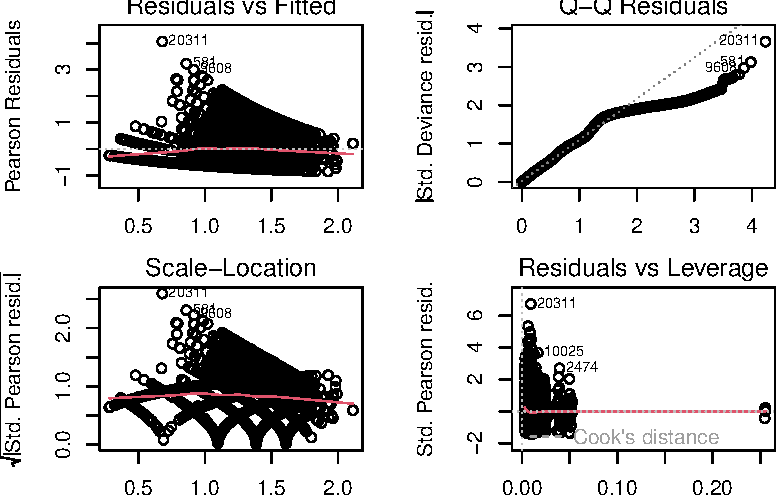
\includegraphics{project_report_files/figure-pdf/unnamed-chunk-11-1.pdf}

}

\end{figure}

Looking at this scatter plot of Yards vs Defenders In The Box, there
appears to be a quadratic function relationship between the two
variables. Therefore, when a reduced model is created, the Defenders In
The Box variable will be squared in order to capture this relationship

\begin{Shaded}
\begin{Highlighting}[]
\CommentTok{\# Scatter plot of yards vs. YardsFromOwnGoal}
\FunctionTok{plot}\NormalTok{(football\_data}\SpecialCharTok{$}\NormalTok{Yards, football\_data}\SpecialCharTok{$}\NormalTok{YardsFromOwnGoal, }\AttributeTok{main =} \StringTok{"Yards vs. Yards From Own Goal"}\NormalTok{, }\AttributeTok{xlab =} \StringTok{"Yards"}\NormalTok{, }\AttributeTok{ylab =} \StringTok{"Yards From Own Goal"}\NormalTok{, }\AttributeTok{pch =} \DecValTok{19}\NormalTok{)}
\end{Highlighting}
\end{Shaded}

\begin{figure}[H]

{\centering \includegraphics{project_report_files/figure-pdf/unnamed-chunk-12-1.pdf}

}

\end{figure}

The scatterplot of Yards vs Yards From Own Goal shows that there is a
linear relationship between the two variables. Therefore, when a reduced
model is created, the Yards From Own Goal variable will not be changed
since the model is already capturing this linear relationship.

In order to capture these relationships between variables, a new, full
model will be synthesized. This model will include the Distance variable
with a sine function and the Defenders In The Box variable squared.
However, the Box-Cox transformation will need to be run again.

\begin{Shaded}
\begin{Highlighting}[]
\NormalTok{lambda\_full }\OtherTok{\textless{}{-}} \FunctionTok{boxcox}\NormalTok{(}\FunctionTok{lm}\NormalTok{(Yards }\SpecialCharTok{\textasciitilde{}}\NormalTok{ Quarter }\SpecialCharTok{+}\NormalTok{ Down }\SpecialCharTok{+} \FunctionTok{sin}\NormalTok{(Distance) }\SpecialCharTok{+}\NormalTok{ OffenseFormation }\SpecialCharTok{+}\NormalTok{ RB }\SpecialCharTok{+}\NormalTok{ TE }\SpecialCharTok{+}\NormalTok{ WR }\SpecialCharTok{+}\NormalTok{ DefendersInTheBox}\SpecialCharTok{\^{}}\DecValTok{2} \SpecialCharTok{+}\NormalTok{ Week }\SpecialCharTok{+}\NormalTok{ GameWeather }\SpecialCharTok{+}\NormalTok{ Temperature }\SpecialCharTok{+}\NormalTok{ Humidity }\SpecialCharTok{+}\NormalTok{ WindSpeed }\SpecialCharTok{+}\NormalTok{ WindDirection }\SpecialCharTok{+}\NormalTok{ GameHour }\SpecialCharTok{+}\NormalTok{ DL }\SpecialCharTok{+}\NormalTok{ LB }\SpecialCharTok{+}\NormalTok{ BL }\SpecialCharTok{+}\NormalTok{ YardsFromOwnGoal }\SpecialCharTok{+}\NormalTok{ ScoreDelta, }\AttributeTok{data =}\NormalTok{ football\_data))}
\end{Highlighting}
\end{Shaded}

\begin{figure}[H]

{\centering \includegraphics{project_report_files/figure-pdf/unnamed-chunk-13-1.pdf}

}

\end{figure}

\begin{Shaded}
\begin{Highlighting}[]
\FunctionTok{summary}\NormalTok{(lambda\_full)}
\end{Highlighting}
\end{Shaded}

\begin{verbatim}
  Length Class  Mode   
x 100    -none- numeric
y 100    -none- numeric
\end{verbatim}

The best lambda value for the Box-Cox tranformation is as follows:

\begin{Shaded}
\begin{Highlighting}[]
\NormalTok{lambda\_full}\SpecialCharTok{$}\NormalTok{x[}\FunctionTok{which.max}\NormalTok{(lambda\_full}\SpecialCharTok{$}\NormalTok{y)]}
\end{Highlighting}
\end{Shaded}

\begin{verbatim}
[1] 0.2222222
\end{verbatim}

Now the Box-Cox tranformation will be applied to the variable Yards with
the best lambda value.

\begin{Shaded}
\begin{Highlighting}[]
\NormalTok{lm\_model\_full }\OtherTok{\textless{}{-}} \FunctionTok{lm}\NormalTok{((Yards}\SpecialCharTok{\^{}}\NormalTok{(lambda\_full}\SpecialCharTok{$}\NormalTok{x[}\FunctionTok{which.max}\NormalTok{(lambda\_full}\SpecialCharTok{$}\NormalTok{y)])) }\SpecialCharTok{\textasciitilde{}}\NormalTok{ Quarter }\SpecialCharTok{+}\NormalTok{ Down }\SpecialCharTok{+} \FunctionTok{sin}\NormalTok{(Distance) }\SpecialCharTok{+}\NormalTok{ OffenseFormation }\SpecialCharTok{+}\NormalTok{ RB }\SpecialCharTok{+}\NormalTok{ TE }\SpecialCharTok{+}\NormalTok{ WR }\SpecialCharTok{+}\NormalTok{ DefendersInTheBox}\SpecialCharTok{\^{}}\DecValTok{2} \SpecialCharTok{+}\NormalTok{ Week }\SpecialCharTok{+}\NormalTok{ GameWeather }\SpecialCharTok{+}\NormalTok{ Temperature }\SpecialCharTok{+}\NormalTok{ Humidity }\SpecialCharTok{+}\NormalTok{ WindSpeed }\SpecialCharTok{+}\NormalTok{ WindDirection }\SpecialCharTok{+}\NormalTok{ GameHour }\SpecialCharTok{+}\NormalTok{ DL }\SpecialCharTok{+}\NormalTok{ LB }\SpecialCharTok{+}\NormalTok{ BL }\SpecialCharTok{+}\NormalTok{ YardsFromOwnGoal }\SpecialCharTok{+}\NormalTok{ ScoreDelta, }\AttributeTok{data =}\NormalTok{ football\_data)}
\FunctionTok{summary}\NormalTok{(lm\_model\_full)}
\end{Highlighting}
\end{Shaded}

\begin{verbatim}

Call:
lm(formula = (Yards^(lambda_full$x[which.max(lambda_full$y)])) ~ 
    Quarter + Down + sin(Distance) + OffenseFormation + RB + 
        TE + WR + DefendersInTheBox^2 + Week + GameWeather + 
        Temperature + Humidity + WindSpeed + WindDirection + 
        GameHour + DL + LB + BL + YardsFromOwnGoal + ScoreDelta, 
    data = football_data)

Residuals:
     Min       1Q   Median       3Q      Max 
-0.42973 -0.13769  0.00597  0.13972  0.46621 

Coefficients:
                             Estimate Std. Error t value Pr(>|t|)    
(Intercept)                 1.577e+00  4.257e-01   3.703 0.000213 ***
Quarter                     4.477e-04  1.127e-03   0.397 0.691071    
Down                        7.903e-04  2.274e-03   0.348 0.728177    
sin(Distance)              -1.343e-02  2.572e-03  -5.223 1.78e-07 ***
OffenseFormationEMPTY       1.855e-02  1.926e-01   0.096 0.923277    
OffenseFormationI_FORM     -1.959e-02  1.885e-01  -0.104 0.917217    
OffenseFormationJUMBO      -1.058e-01  1.887e-01  -0.560 0.575249    
OffenseFormationPISTOL     -1.803e-02  1.885e-01  -0.096 0.923833    
OffenseFormationSHOTGUN    -3.093e-02  1.884e-01  -0.164 0.869618    
OffenseFormationSINGLEBACK -2.134e-02  1.884e-01  -0.113 0.909848    
OffenseFormationUNKNOWN    -4.476e-02  2.107e-01  -0.212 0.831757    
OffenseFormationWILDCAT    -2.276e-03  1.901e-01  -0.012 0.990445    
RB                         -3.043e-03  5.907e-03  -0.515 0.606408    
TE                         -2.328e-04  4.921e-03  -0.047 0.962266    
WR                         -6.469e-03  5.016e-03  -1.290 0.197211    
DefendersInTheBox          -2.954e-02  1.942e-03 -15.214  < 2e-16 ***
Week                       -2.368e-04  3.461e-04  -0.684 0.493767    
GameWeathernone             7.371e-03  4.264e-03   1.729 0.083870 .  
GameWeatherovercast        -7.788e-04  3.134e-03  -0.248 0.803755    
GameWeatherrain            -4.390e-03  6.351e-03  -0.691 0.489464    
GameWeathersnow            -1.081e-02  1.847e-02  -0.585 0.558466    
Temperature                -3.118e-04  1.014e-04  -3.074 0.002115 ** 
Humidity                   -3.784e-05  6.340e-05  -0.597 0.550599    
WindSpeed                   5.225e-05  3.120e-04   0.167 0.867002    
WindDirectionnone          -1.063e-02  8.185e-03  -1.298 0.194240    
WindDirectionnorth         -4.787e-03  9.564e-03  -0.501 0.616690    
WindDirectionnorth east    -8.309e-03  8.238e-03  -1.009 0.313158    
WindDirectionnorth west    -5.569e-03  8.320e-03  -0.669 0.503289    
WindDirectionsouth         -8.639e-03  9.055e-03  -0.954 0.340025    
WindDirectionsouth east    -4.528e-03  8.577e-03  -0.528 0.597521    
WindDirectionsouth west    -6.451e-03  8.079e-03  -0.798 0.424624    
WindDirectionwest          -4.237e-03  9.653e-03  -0.439 0.660729    
GameHour                    4.356e-04  2.931e-04   1.486 0.137242    
DL                         -1.601e-03  3.465e-02  -0.046 0.963145    
LB                         -1.855e-03  3.473e-02  -0.053 0.957403    
BL                          6.786e-03  3.473e-02   0.195 0.845108    
YardsFromOwnGoal           -4.841e-04  5.231e-05  -9.256  < 2e-16 ***
ScoreDelta                 -2.135e-04  1.211e-04  -1.763 0.077874 .  
---
Signif. codes:  0 '***' 0.001 '**' 0.01 '*' 0.05 '.' 0.1 ' ' 1

Residual standard error: 0.1883 on 21584 degrees of freedom
  (279 observations deleted due to missingness)
Multiple R-squared:  0.04437,   Adjusted R-squared:  0.04273 
F-statistic: 27.08 on 37 and 21584 DF,  p-value: < 2.2e-16
\end{verbatim}

Now lets use the step function to find the best model for the data.

\begin{Shaded}
\begin{Highlighting}[]
\NormalTok{lm\_model\_step }\OtherTok{\textless{}{-}} \FunctionTok{invisible}\NormalTok{(}\FunctionTok{step}\NormalTok{(lm\_model\_full, }\AttributeTok{direction =} \StringTok{"backward"}\NormalTok{))}
\end{Highlighting}
\end{Shaded}

\begin{verbatim}
Start:  AIC=-72165.49
(Yards^(lambda_full$x[which.max(lambda_full$y)])) ~ Quarter + 
    Down + sin(Distance) + OffenseFormation + RB + TE + WR + 
    DefendersInTheBox^2 + Week + GameWeather + Temperature + 
    Humidity + WindSpeed + WindDirection + GameHour + DL + LB + 
    BL + YardsFromOwnGoal + ScoreDelta

                    Df Sum of Sq    RSS    AIC
- WindDirection      8    0.1190 765.49 -72178
- GameWeather        4    0.1523 765.52 -72169
- DL                 1    0.0001 765.37 -72167
- TE                 1    0.0001 765.37 -72167
- LB                 1    0.0001 765.37 -72167
- WindSpeed          1    0.0010 765.37 -72167
- BL                 1    0.0014 765.37 -72167
- Down               1    0.0043 765.37 -72167
- Quarter            1    0.0056 765.37 -72167
- RB                 1    0.0094 765.38 -72167
- Humidity           1    0.0126 765.38 -72167
- Week               1    0.0166 765.38 -72167
- WR                 1    0.0590 765.43 -72166
<none>                           765.37 -72165
- GameHour           1    0.0783 765.45 -72165
- ScoreDelta         1    0.1102 765.48 -72164
- Temperature        1    0.3351 765.70 -72158
- sin(Distance)      1    0.9674 766.33 -72140
- OffenseFormation   8    2.9885 768.36 -72097
- YardsFromOwnGoal   1    3.0380 768.41 -72082
- DefendersInTheBox  1    8.2081 773.58 -71937

Step:  AIC=-72178.13
(Yards^(lambda_full$x[which.max(lambda_full$y)])) ~ Quarter + 
    Down + sin(Distance) + OffenseFormation + RB + TE + WR + 
    DefendersInTheBox + Week + GameWeather + Temperature + Humidity + 
    WindSpeed + GameHour + DL + LB + BL + YardsFromOwnGoal + 
    ScoreDelta

                    Df Sum of Sq    RSS    AIC
- GameWeather        4    0.1167 765.60 -72183
- DL                 1    0.0001 765.49 -72180
- LB                 1    0.0001 765.49 -72180
- TE                 1    0.0001 765.49 -72180
- BL                 1    0.0014 765.49 -72180
- Down               1    0.0037 765.49 -72180
- Humidity           1    0.0042 765.49 -72180
- Quarter            1    0.0055 765.49 -72180
- RB                 1    0.0090 765.50 -72180
- Week               1    0.0116 765.50 -72180
- WindSpeed          1    0.0137 765.50 -72180
- WR                 1    0.0605 765.55 -72178
<none>                           765.49 -72178
- GameHour           1    0.0790 765.57 -72178
- ScoreDelta         1    0.1080 765.59 -72177
- Temperature        1    0.3070 765.79 -72171
- sin(Distance)      1    0.9619 766.45 -72153
- OffenseFormation   8    3.0060 768.49 -72109
- YardsFromOwnGoal   1    3.0296 768.52 -72095
- DefendersInTheBox  1    8.2167 773.70 -71949

Step:  AIC=-72182.83
(Yards^(lambda_full$x[which.max(lambda_full$y)])) ~ Quarter + 
    Down + sin(Distance) + OffenseFormation + RB + TE + WR + 
    DefendersInTheBox + Week + Temperature + Humidity + WindSpeed + 
    GameHour + DL + LB + BL + YardsFromOwnGoal + ScoreDelta

                    Df Sum of Sq    RSS    AIC
- DL                 1    0.0001 765.60 -72185
- WindSpeed          1    0.0001 765.60 -72185
- LB                 1    0.0001 765.60 -72185
- TE                 1    0.0002 765.60 -72185
- BL                 1    0.0015 765.60 -72185
- Down               1    0.0036 765.61 -72185
- Quarter            1    0.0054 765.61 -72185
- RB                 1    0.0078 765.61 -72185
- Week               1    0.0105 765.61 -72185
- Humidity           1    0.0541 765.66 -72183
- WR                 1    0.0624 765.67 -72183
<none>                           765.60 -72183
- GameHour           1    0.0797 765.68 -72183
- ScoreDelta         1    0.1043 765.71 -72182
- Temperature        1    0.2870 765.89 -72177
- sin(Distance)      1    0.9577 766.56 -72158
- OffenseFormation   8    3.0075 768.61 -72114
- YardsFromOwnGoal   1    3.0221 768.63 -72100
- DefendersInTheBox  1    8.2362 773.84 -71953

Step:  AIC=-72184.83
(Yards^(lambda_full$x[which.max(lambda_full$y)])) ~ Quarter + 
    Down + sin(Distance) + OffenseFormation + RB + TE + WR + 
    DefendersInTheBox + Week + Temperature + Humidity + WindSpeed + 
    GameHour + LB + BL + YardsFromOwnGoal + ScoreDelta

                    Df Sum of Sq    RSS    AIC
- WindSpeed          1    0.0001 765.60 -72187
- TE                 1    0.0002 765.60 -72187
- LB                 1    0.0020 765.61 -72187
- Down               1    0.0036 765.61 -72187
- Quarter            1    0.0054 765.61 -72187
- RB                 1    0.0078 765.61 -72187
- Week               1    0.0105 765.61 -72187
- Humidity           1    0.0541 765.66 -72185
- WR                 1    0.0625 765.67 -72185
<none>                           765.60 -72185
- GameHour           1    0.0797 765.68 -72185
- ScoreDelta         1    0.1045 765.71 -72184
- BL                 1    0.2507 765.85 -72180
- Temperature        1    0.2869 765.89 -72179
- sin(Distance)      1    0.9577 766.56 -72160
- OffenseFormation   8    3.0202 768.62 -72116
- YardsFromOwnGoal   1    3.0230 768.63 -72102
- DefendersInTheBox  1    8.2564 773.86 -71955

Step:  AIC=-72186.83
(Yards^(lambda_full$x[which.max(lambda_full$y)])) ~ Quarter + 
    Down + sin(Distance) + OffenseFormation + RB + TE + WR + 
    DefendersInTheBox + Week + Temperature + Humidity + GameHour + 
    LB + BL + YardsFromOwnGoal + ScoreDelta

                    Df Sum of Sq    RSS    AIC
- TE                 1    0.0002 765.60 -72189
- LB                 1    0.0020 765.61 -72189
- Down               1    0.0036 765.61 -72189
- Quarter            1    0.0054 765.61 -72189
- RB                 1    0.0078 765.61 -72189
- Week               1    0.0106 765.61 -72189
- Humidity           1    0.0560 765.66 -72187
- WR                 1    0.0625 765.67 -72187
<none>                           765.60 -72187
- GameHour           1    0.0797 765.68 -72187
- ScoreDelta         1    0.1045 765.71 -72186
- BL                 1    0.2507 765.85 -72182
- Temperature        1    0.2927 765.90 -72181
- sin(Distance)      1    0.9578 766.56 -72162
- OffenseFormation   8    3.0202 768.62 -72118
- YardsFromOwnGoal   1    3.0246 768.63 -72104
- DefendersInTheBox  1    8.2563 773.86 -71957

Step:  AIC=-72188.82
(Yards^(lambda_full$x[which.max(lambda_full$y)])) ~ Quarter + 
    Down + sin(Distance) + OffenseFormation + RB + WR + DefendersInTheBox + 
    Week + Temperature + Humidity + GameHour + LB + BL + YardsFromOwnGoal + 
    ScoreDelta

                    Df Sum of Sq    RSS    AIC
- LB                 1    0.0020 765.61 -72191
- Down               1    0.0036 765.61 -72191
- Quarter            1    0.0054 765.61 -72191
- Week               1    0.0105 765.61 -72191
- RB                 1    0.0125 765.62 -72190
- Humidity           1    0.0559 765.66 -72189
<none>                           765.60 -72189
- GameHour           1    0.0796 765.68 -72189
- ScoreDelta         1    0.1047 765.71 -72188
- WR                 1    0.2064 765.81 -72185
- BL                 1    0.2506 765.85 -72184
- Temperature        1    0.2929 765.90 -72183
- sin(Distance)      1    0.9577 766.56 -72164
- OffenseFormation   8    3.1049 768.71 -72117
- YardsFromOwnGoal   1    3.0249 768.63 -72106
- DefendersInTheBox  1    8.2660 773.87 -71959

Step:  AIC=-72190.77
(Yards^(lambda_full$x[which.max(lambda_full$y)])) ~ Quarter + 
    Down + sin(Distance) + OffenseFormation + RB + WR + DefendersInTheBox + 
    Week + Temperature + Humidity + GameHour + BL + YardsFromOwnGoal + 
    ScoreDelta

                    Df Sum of Sq    RSS    AIC
- Down               1    0.0036 765.61 -72193
- Quarter            1    0.0054 765.61 -72193
- Week               1    0.0097 765.62 -72192
- RB                 1    0.0124 765.62 -72192
- Humidity           1    0.0562 765.66 -72191
<none>                           765.61 -72191
- GameHour           1    0.0797 765.69 -72191
- ScoreDelta         1    0.1038 765.71 -72190
- WR                 1    0.2056 765.81 -72187
- Temperature        1    0.2910 765.90 -72185
- BL                 1    0.2955 765.90 -72184
- sin(Distance)      1    0.9574 766.56 -72166
- OffenseFormation   8    3.1036 768.71 -72119
- YardsFromOwnGoal   1    3.0231 768.63 -72108
- DefendersInTheBox  1    8.2755 773.88 -71960

Step:  AIC=-72192.67
(Yards^(lambda_full$x[which.max(lambda_full$y)])) ~ Quarter + 
    sin(Distance) + OffenseFormation + RB + WR + DefendersInTheBox + 
    Week + Temperature + Humidity + GameHour + BL + YardsFromOwnGoal + 
    ScoreDelta

                    Df Sum of Sq    RSS    AIC
- Quarter            1    0.0057 765.61 -72195
- Week               1    0.0096 765.62 -72194
- RB                 1    0.0125 765.62 -72194
- Humidity           1    0.0563 765.67 -72193
<none>                           765.61 -72193
- GameHour           1    0.0780 765.69 -72192
- ScoreDelta         1    0.1043 765.71 -72192
- WR                 1    0.2080 765.82 -72189
- Temperature        1    0.2909 765.90 -72186
- BL                 1    0.3023 765.91 -72186
- sin(Distance)      1    1.1972 766.81 -72161
- OffenseFormation   8    3.1001 768.71 -72121
- YardsFromOwnGoal   1    3.0230 768.63 -72109
- DefendersInTheBox  1    8.2775 773.89 -71962

Step:  AIC=-72194.51
(Yards^(lambda_full$x[which.max(lambda_full$y)])) ~ sin(Distance) + 
    OffenseFormation + RB + WR + DefendersInTheBox + Week + Temperature + 
    Humidity + GameHour + BL + YardsFromOwnGoal + ScoreDelta

                    Df Sum of Sq    RSS    AIC
- Week               1    0.0098 765.62 -72196
- RB                 1    0.0128 765.63 -72196
- Humidity           1    0.0566 765.67 -72195
<none>                           765.61 -72195
- GameHour           1    0.0770 765.69 -72194
- ScoreDelta         1    0.1023 765.72 -72194
- WR                 1    0.2101 765.82 -72191
- Temperature        1    0.2913 765.91 -72188
- BL                 1    0.3048 765.92 -72188
- sin(Distance)      1    1.1968 766.81 -72163
- OffenseFormation   8    3.1018 768.72 -72123
- YardsFromOwnGoal   1    3.0176 768.63 -72111
- DefendersInTheBox  1    8.2741 773.89 -71964

Step:  AIC=-72196.23
(Yards^(lambda_full$x[which.max(lambda_full$y)])) ~ sin(Distance) + 
    OffenseFormation + RB + WR + DefendersInTheBox + Temperature + 
    Humidity + GameHour + BL + YardsFromOwnGoal + ScoreDelta

                    Df Sum of Sq    RSS    AIC
- RB                 1    0.0129 765.64 -72198
- Humidity           1    0.0525 765.68 -72197
<none>                           765.62 -72196
- GameHour           1    0.0768 765.70 -72196
- ScoreDelta         1    0.1045 765.73 -72195
- WR                 1    0.2132 765.84 -72192
- BL                 1    0.3046 765.93 -72190
- Temperature        1    0.3711 766.00 -72188
- sin(Distance)      1    1.1993 766.82 -72164
- OffenseFormation   8    3.1001 768.72 -72125
- YardsFromOwnGoal   1    3.0118 768.64 -72113
- DefendersInTheBox  1    8.2992 773.92 -71965

Step:  AIC=-72197.86
(Yards^(lambda_full$x[which.max(lambda_full$y)])) ~ sin(Distance) + 
    OffenseFormation + WR + DefendersInTheBox + Temperature + 
    Humidity + GameHour + BL + YardsFromOwnGoal + ScoreDelta

                    Df Sum of Sq    RSS    AIC
- Humidity           1    0.0507 765.69 -72198
<none>                           765.64 -72198
- GameHour           1    0.0767 765.71 -72198
- ScoreDelta         1    0.1034 765.74 -72197
- WR                 1    0.2002 765.84 -72194
- BL                 1    0.3010 765.94 -72191
- Temperature        1    0.3715 766.01 -72189
- sin(Distance)      1    1.2007 766.84 -72166
- OffenseFormation   8    3.0880 768.73 -72127
- YardsFromOwnGoal   1    3.0219 768.66 -72115
- DefendersInTheBox  1    8.2919 773.93 -71967

Step:  AIC=-72198.43
(Yards^(lambda_full$x[which.max(lambda_full$y)])) ~ sin(Distance) + 
    OffenseFormation + WR + DefendersInTheBox + Temperature + 
    GameHour + BL + YardsFromOwnGoal + ScoreDelta

                    Df Sum of Sq    RSS    AIC
<none>                           765.69 -72198
- GameHour           1    0.0750 765.76 -72198
- ScoreDelta         1    0.0968 765.78 -72198
- WR                 1    0.1959 765.88 -72195
- BL                 1    0.3006 765.99 -72192
- Temperature        1    0.3305 766.02 -72191
- sin(Distance)      1    1.1971 766.89 -72167
- OffenseFormation   8    3.1087 768.80 -72127
- YardsFromOwnGoal   1    3.0339 768.72 -72115
- DefendersInTheBox  1    8.2601 773.95 -71968
\end{verbatim}

\begin{Shaded}
\begin{Highlighting}[]
\FunctionTok{summary}\NormalTok{(lm\_model\_step)}
\end{Highlighting}
\end{Shaded}

\begin{verbatim}

Call:
lm(formula = (Yards^(lambda_full$x[which.max(lambda_full$y)])) ~ 
    sin(Distance) + OffenseFormation + WR + DefendersInTheBox + 
        Temperature + GameHour + BL + YardsFromOwnGoal + ScoreDelta, 
    data = football_data)

Residuals:
     Min       1Q   Median       3Q      Max 
-0.41862 -0.13809  0.00558  0.13957  0.46668 

Coefficients:
                             Estimate Std. Error t value Pr(>|t|)    
(Intercept)                 1.539e+00  1.897e-01   8.114 5.18e-16 ***
sin(Distance)              -1.295e-02  2.229e-03  -5.812 6.26e-09 ***
OffenseFormationEMPTY       1.762e-02  1.925e-01   0.092  0.92706    
OffenseFormationI_FORM     -2.276e-02  1.883e-01  -0.121  0.90379    
OffenseFormationJUMBO      -1.084e-01  1.886e-01  -0.575  0.56552    
OffenseFormationPISTOL     -2.057e-02  1.884e-01  -0.109  0.91305    
OffenseFormationSHOTGUN    -3.253e-02  1.883e-01  -0.173  0.86282    
OffenseFormationSINGLEBACK -2.264e-02  1.883e-01  -0.120  0.90430    
OffenseFormationUNKNOWN    -4.777e-02  2.105e-01  -0.227  0.82048    
OffenseFormationWILDCAT    -5.954e-03  1.899e-01  -0.031  0.97499    
WR                         -5.969e-03  2.539e-03  -2.351  0.01874 *  
DefendersInTheBox          -2.938e-02  1.924e-03 -15.267  < 2e-16 ***
Temperature                -2.282e-04  7.473e-05  -3.054  0.00226 ** 
GameHour                    4.255e-04  2.924e-04   1.455  0.14563    
BL                          8.703e-03  2.988e-03   2.912  0.00359 ** 
YardsFromOwnGoal           -4.821e-04  5.210e-05  -9.252  < 2e-16 ***
ScoreDelta                 -1.982e-04  1.199e-04  -1.652  0.09847 .  
---
Signif. codes:  0 '***' 0.001 '**' 0.01 '*' 0.05 '.' 0.1 ' ' 1

Residual standard error: 0.1883 on 21605 degrees of freedom
  (279 observations deleted due to missingness)
Multiple R-squared:  0.04397,   Adjusted R-squared:  0.04326 
F-statistic:  62.1 on 16 and 21605 DF,  p-value: < 2.2e-16
\end{verbatim}

This new reduced model needs to be run similar to that of the previous
models utilizing the Box-Cox transformation.

\begin{Shaded}
\begin{Highlighting}[]
\NormalTok{lambda\_reduced }\OtherTok{\textless{}{-}} \FunctionTok{boxcox}\NormalTok{(}\FunctionTok{lm}\NormalTok{(Yards }\SpecialCharTok{\textasciitilde{}} \FunctionTok{sin}\NormalTok{(Distance) }\SpecialCharTok{+}\NormalTok{ WR }\SpecialCharTok{+}\NormalTok{ DefendersInTheBox}\SpecialCharTok{\^{}}\DecValTok{2} \SpecialCharTok{+}\NormalTok{ Temperature }\SpecialCharTok{+}\NormalTok{ BL }\SpecialCharTok{+}\NormalTok{ YardsFromOwnGoal, }\AttributeTok{data =}\NormalTok{ football\_data))}
\end{Highlighting}
\end{Shaded}

\begin{figure}[H]

{\centering \includegraphics{project_report_files/figure-pdf/unnamed-chunk-17-1.pdf}

}

\end{figure}

The best lambda value for the Box-Cox tranformation is as follows:

\begin{Shaded}
\begin{Highlighting}[]
\NormalTok{lambda\_reduced}\SpecialCharTok{$}\NormalTok{x[}\FunctionTok{which.max}\NormalTok{(lambda\_reduced}\SpecialCharTok{$}\NormalTok{y)]}
\end{Highlighting}
\end{Shaded}

\begin{verbatim}
[1] 0.2222222
\end{verbatim}

Now the Box-Cox tranformation will be applied to the variable Yards with
the best lambda value.

\begin{Shaded}
\begin{Highlighting}[]
\NormalTok{lm\_model\_reduced }\OtherTok{\textless{}{-}} \FunctionTok{lm}\NormalTok{((Yards}\SpecialCharTok{\^{}}\NormalTok{(lambda\_reduced}\SpecialCharTok{$}\NormalTok{x[}\FunctionTok{which.max}\NormalTok{(lambda\_reduced}\SpecialCharTok{$}\NormalTok{y)])) }\SpecialCharTok{\textasciitilde{}} \FunctionTok{sin}\NormalTok{(Distance) }\SpecialCharTok{+}\NormalTok{ WR }\SpecialCharTok{+}\NormalTok{ DefendersInTheBox}\SpecialCharTok{\^{}}\DecValTok{2} \SpecialCharTok{+}\NormalTok{ Temperature }\SpecialCharTok{+}\NormalTok{ BL }\SpecialCharTok{+}\NormalTok{ YardsFromOwnGoal, }\AttributeTok{data =}\NormalTok{ football\_data)}
\FunctionTok{summary}\NormalTok{(lm\_model\_reduced)}
\end{Highlighting}
\end{Shaded}

\begin{verbatim}

Call:
lm(formula = (Yards^(lambda_reduced$x[which.max(lambda_reduced$y)])) ~ 
    sin(Distance) + WR + DefendersInTheBox^2 + Temperature + 
        BL + YardsFromOwnGoal, data = football_data)

Residuals:
     Min       1Q   Median       3Q      Max 
-0.42943 -0.13845  0.00666  0.14017  0.44016 

Coefficients:
                    Estimate Std. Error t value Pr(>|t|)    
(Intercept)        1.520e+00  2.267e-02  67.020  < 2e-16 ***
sin(Distance)     -1.571e-02  2.212e-03  -7.100 1.28e-12 ***
WR                -5.485e-03  2.422e-03  -2.265  0.02354 *  
DefendersInTheBox -3.058e-02  1.877e-03 -16.295  < 2e-16 ***
Temperature       -2.305e-04  7.483e-05  -3.080  0.00208 ** 
BL                 9.652e-03  2.957e-03   3.264  0.00110 ** 
YardsFromOwnGoal  -5.365e-04  5.169e-05 -10.380  < 2e-16 ***
---
Signif. codes:  0 '***' 0.001 '**' 0.01 '*' 0.05 '.' 0.1 ' ' 1

Residual standard error: 0.1886 on 21615 degrees of freedom
  (279 observations deleted due to missingness)
Multiple R-squared:  0.03983,   Adjusted R-squared:  0.03956 
F-statistic: 149.4 on 6 and 21615 DF,  p-value: < 2.2e-16
\end{verbatim}

By creating a Residuals vs Fitted plot, a Q-Q Residuals plot, a
Scale-Location plot, and a Residuals vs Leverage plot, the assumptions
of the model can be checked.

\begin{Shaded}
\begin{Highlighting}[]
\FunctionTok{par}\NormalTok{(}\AttributeTok{mfrow =} \FunctionTok{c}\NormalTok{(}\DecValTok{2}\NormalTok{, }\DecValTok{2}\NormalTok{))}
\NormalTok{old.par }\OtherTok{=} \FunctionTok{par}\NormalTok{(}\AttributeTok{mar =} \FunctionTok{c}\NormalTok{(}\DecValTok{3}\NormalTok{, }\DecValTok{4}\NormalTok{, }\DecValTok{1}\NormalTok{, }\DecValTok{2}\NormalTok{))}
\FunctionTok{plot}\NormalTok{(lm\_model\_reduced)}
\end{Highlighting}
\end{Shaded}

\begin{figure}[H]

{\centering 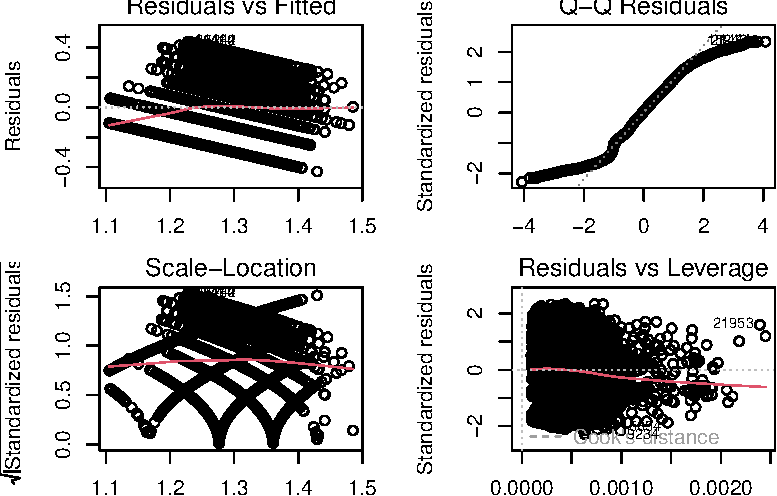
\includegraphics{project_report_files/figure-pdf/unnamed-chunk-20-1.pdf}

}

\end{figure}

Based on the plots above, the normality assumption is not violated, as
the Q-Q Residuals plot shows that the residuals are mainly normally
distributed.

In order to gain a better understanding of how these variables affect
the predicted yards, scatter plots of the predicted yards versus each of
the predictors will be created. However, the only scatter plots that
will be synthesized are those that have the three highest t values:
Distance, DefendersInTheBox, and YardsFromOwnGoal.

\begin{Shaded}
\begin{Highlighting}[]
\NormalTok{football\_data}\SpecialCharTok{$}\NormalTok{predicted\_yards }\OtherTok{\textless{}{-}} \FunctionTok{predict}\NormalTok{(lm\_model\_reduced, football\_data)}
\end{Highlighting}
\end{Shaded}

\begin{Shaded}
\begin{Highlighting}[]
\CommentTok{\# Scatter plot of predicted yards vs. Distance}
\FunctionTok{plot}\NormalTok{(football\_data}\SpecialCharTok{$}\NormalTok{predicted\_yards, football\_data}\SpecialCharTok{$}\NormalTok{Distance, }\AttributeTok{main =} \StringTok{"Predicted Yards vs. Distance"}\NormalTok{, }\AttributeTok{xlab =} \StringTok{"Predicted Yards"}\NormalTok{, }\AttributeTok{ylab =} \StringTok{"Distance"}\NormalTok{, }\AttributeTok{pch =} \DecValTok{19}\NormalTok{)}
\FunctionTok{abline}\NormalTok{(}\DecValTok{0}\NormalTok{, }\DecValTok{1}\NormalTok{, }\AttributeTok{col =} \StringTok{"red"}\NormalTok{)  }\CommentTok{\# Adds a 45{-}degree line}
\end{Highlighting}
\end{Shaded}

\begin{figure}[H]

{\centering \includegraphics{project_report_files/figure-pdf/unnamed-chunk-22-1.pdf}

}

\end{figure}

\begin{Shaded}
\begin{Highlighting}[]
\CommentTok{\# Scatter plot of predicted yards vs. DefendersInTheBox}
\FunctionTok{plot}\NormalTok{(football\_data}\SpecialCharTok{$}\NormalTok{predicted\_yards, football\_data}\SpecialCharTok{$}\NormalTok{DefendersInTheBox, }\AttributeTok{main =} \StringTok{"Predicted Yards vs. DefendersInTheBox"}\NormalTok{, }\AttributeTok{xlab =} \StringTok{"Predicted Yards"}\NormalTok{, }\AttributeTok{ylab =} \StringTok{"DefendersInTheBox"}\NormalTok{, }\AttributeTok{pch =} \DecValTok{19}\NormalTok{)}
\FunctionTok{abline}\NormalTok{(}\DecValTok{0}\NormalTok{, }\DecValTok{1}\NormalTok{, }\AttributeTok{col =} \StringTok{"red"}\NormalTok{)  }\CommentTok{\# Adds a 45{-}degree line}
\end{Highlighting}
\end{Shaded}

\begin{figure}[H]

{\centering \includegraphics{project_report_files/figure-pdf/unnamed-chunk-23-1.pdf}

}

\end{figure}

\begin{Shaded}
\begin{Highlighting}[]
\CommentTok{\# Scatter plot of predicted yards vs. YardsFromOwnGoal}
\FunctionTok{plot}\NormalTok{(football\_data}\SpecialCharTok{$}\NormalTok{predicted\_yards, football\_data}\SpecialCharTok{$}\NormalTok{YardsFromOwnGoal, }\AttributeTok{main =} \StringTok{"Predicted Yards vs. YardsFromOwnGoal"}\NormalTok{, }\AttributeTok{xlab =} \StringTok{"Predicted Yards"}\NormalTok{, }\AttributeTok{ylab =} \StringTok{"YardsFromOwnGoal"}\NormalTok{, }\AttributeTok{pch =} \DecValTok{19}\NormalTok{)}
\FunctionTok{abline}\NormalTok{(}\DecValTok{0}\NormalTok{, }\DecValTok{1}\NormalTok{, }\AttributeTok{col =} \StringTok{"red"}\NormalTok{)  }\CommentTok{\# Adds a 45{-}degree line}
\end{Highlighting}
\end{Shaded}

\begin{figure}[H]

{\centering \includegraphics{project_report_files/figure-pdf/unnamed-chunk-24-1.pdf}

}

\end{figure}

\hypertarget{glm-with-gamma-response}{%
\section{GLM with Gamma Response}\label{glm-with-gamma-response}}

The next model that will be synthesized is a GLM with a gamma response.
The gamma distribution is a two-parameter family of continuous
probability distributions. The gamma distribution is a generalization of
the exponential distribution. The gamma distribution is frequently used
to model right-skewed data. The gamma distribution is a two-parameter
family of continuous probability distributions. The gamma distribution
is a generalization of the exponential distribution. The gamma
distribution is frequently used to model right-skewed data. The gamma
distribution is a two-parameter family of continuous probability
distributions. The gamma distribution is a generalization of the
exponential distribution. The gamma distribution is frequently used to
model right-skewed data. The gamma distribution is a two-parameter
family of continuous probability distributions. The gamma distribution
is a generalization of the exponential distribution. The gamma
distribution is frequently used to model right-skewed data. The gamma
distribution is a two-parameter family of continuous probability
distributions. The gamma distribution is a generalization of the
exponential distribution. The gamma distribution is frequently used to
model right-skewed data. The gamma distribution is a two-parameter
family of continuous probability distributions. The gamma distribution
is a generalization of the exponential distribution. The gamma
distribution is frequently used to model right-skewed data.

Lets start by removing any rows whose yards column is negative. This is
because the gamma distribution cannot have negative values.

\begin{Shaded}
\begin{Highlighting}[]
\CommentTok{\# Remove any rows whose yards column is negative}
\NormalTok{football\_data }\OtherTok{\textless{}{-}}\NormalTok{ football\_data[football\_data}\SpecialCharTok{$}\NormalTok{Yards }\SpecialCharTok{\textgreater{}=} \FloatTok{0.1}\NormalTok{, ]}
\NormalTok{football\_data }\OtherTok{\textless{}{-}}\NormalTok{ football\_data[football\_data}\SpecialCharTok{$}\NormalTok{Yards }\SpecialCharTok{\textless{}=} \DecValTok{10}\NormalTok{, ]}
\end{Highlighting}
\end{Shaded}

\begin{Shaded}
\begin{Highlighting}[]
\CommentTok{\# Fit the model}
\NormalTok{glm\_model\_gamma }\OtherTok{\textless{}{-}} \FunctionTok{glm}\NormalTok{(Yards }\SpecialCharTok{\textasciitilde{}}\NormalTok{ ., }\AttributeTok{data =}\NormalTok{ football\_data, }\AttributeTok{family =} \FunctionTok{Gamma}\NormalTok{(}\AttributeTok{link =} \StringTok{"log"}\NormalTok{))}
\end{Highlighting}
\end{Shaded}

Now lets use the step function to find the best model for the data.

\begin{Shaded}
\begin{Highlighting}[]
\CommentTok{\#glm\_model\_step \textless{}{-} step(glm\_model\_gamma, direction = "backward")}
\CommentTok{\# summary(glm\_model\_step)}
\end{Highlighting}
\end{Shaded}

Running this reduced model yields the following results:

\begin{Shaded}
\begin{Highlighting}[]
\NormalTok{reduced\_model }\OtherTok{\textless{}{-}} \FunctionTok{glm}\NormalTok{(Yards }\SpecialCharTok{\textasciitilde{}}\NormalTok{ YardsFromOwnGoal }\SpecialCharTok{+}\NormalTok{ Distance }\SpecialCharTok{+}\NormalTok{ RB }\SpecialCharTok{+}\NormalTok{ WR }\SpecialCharTok{+}\NormalTok{ DefendersInTheBox }\SpecialCharTok{+}\NormalTok{ BL, }\AttributeTok{data=}\NormalTok{football\_data, }\AttributeTok{family =} \FunctionTok{Gamma}\NormalTok{(}\AttributeTok{link =} \StringTok{"log"}\NormalTok{))}
\FunctionTok{summary}\NormalTok{(reduced\_model)}
\end{Highlighting}
\end{Shaded}

\begin{verbatim}

Call:
glm(formula = Yards ~ YardsFromOwnGoal + Distance + RB + WR + 
    DefendersInTheBox + BL, family = Gamma(link = "log"), data = football_data)

Coefficients:
                    Estimate Std. Error t value Pr(>|t|)    
(Intercept)        1.8518606  0.0767537  24.127  < 2e-16 ***
YardsFromOwnGoal  -0.0015937  0.0001702  -9.365  < 2e-16 ***
Distance           0.0122863  0.0011656  10.541  < 2e-16 ***
RB                 0.0008371  0.0112653   0.074 0.940768    
WR                -0.0143714  0.0082703  -1.738 0.082276 .  
DefendersInTheBox -0.0945131  0.0061146 -15.457  < 2e-16 ***
BL                 0.0328700  0.0095367   3.447 0.000569 ***
---
Signif. codes:  0 '***' 0.001 '**' 0.01 '*' 0.05 '.' 0.1 ' ' 1

(Dispersion parameter for Gamma family taken to be 0.3702443)

    Null deviance: 9063.4  on 21621  degrees of freedom
Residual deviance: 8725.7  on 21615  degrees of freedom
  (279 observations deleted due to missingness)
AIC: 92734

Number of Fisher Scoring iterations: 5
\end{verbatim}

By creating a Residuals vs Fitted plot, a Q-Q Residuals plot, a
Scale-Location plot, and a Residuals vs Leverage plot, the assumptions
of the model can be checked.

\begin{Shaded}
\begin{Highlighting}[]
\FunctionTok{par}\NormalTok{(}\AttributeTok{mfrow =} \FunctionTok{c}\NormalTok{(}\DecValTok{2}\NormalTok{, }\DecValTok{2}\NormalTok{))}
\NormalTok{old.par }\OtherTok{=} \FunctionTok{par}\NormalTok{(}\AttributeTok{mar =} \FunctionTok{c}\NormalTok{(}\DecValTok{3}\NormalTok{, }\DecValTok{4}\NormalTok{, }\DecValTok{1}\NormalTok{, }\DecValTok{2}\NormalTok{))}
\FunctionTok{plot}\NormalTok{(glm\_model\_gamma)}
\end{Highlighting}
\end{Shaded}

\begin{verbatim}
Warning: not plotting observations with leverage one:
  19377
\end{verbatim}

\begin{figure}[H]

{\centering 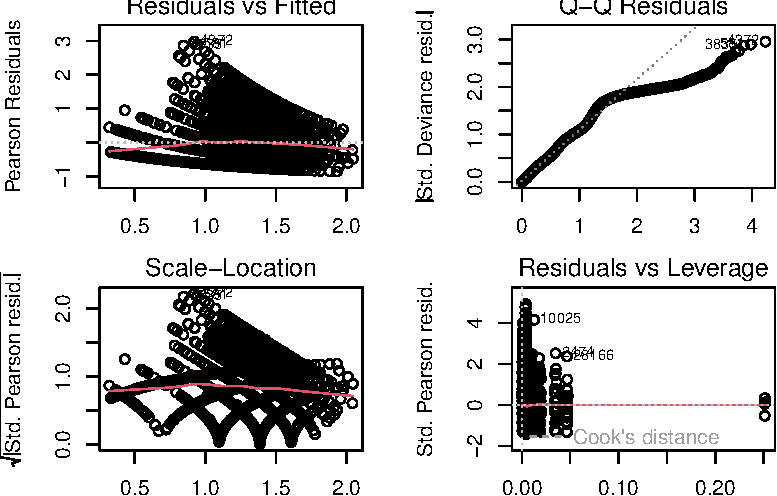
\includegraphics{project_report_files/figure-pdf/unnamed-chunk-29-1.pdf}

}

\end{figure}

\hypertarget{xgboost-model}{%
\section{XGBoost Model}\label{xgboost-model}}

Moving now into the XGBoost model, the data was split into a training
set and a testing set in order to evaluate performance metrics. The
training set will be used to train the model, while the testing set will
be used to test the model. The training set will be 80\% of the data,
while the testing set will be 20\% of the data and randomly selected.

\begin{Shaded}
\begin{Highlighting}[]
\FunctionTok{library}\NormalTok{(fastDummies)}
\end{Highlighting}
\end{Shaded}

\begin{verbatim}
Thank you for using fastDummies!
\end{verbatim}

\begin{verbatim}
To acknowledge our work, please cite the package:
\end{verbatim}

\begin{verbatim}
Kaplan, J. & Schlegel, B. (2023). fastDummies: Fast Creation of Dummy (Binary) Columns and Rows from Categorical Variables. Version 1.7.1. URL: https://github.com/jacobkap/fastDummies, https://jacobkap.github.io/fastDummies/.
\end{verbatim}

\begin{Shaded}
\begin{Highlighting}[]
\CommentTok{\# Convert specified factor columns to dummy variables}
\NormalTok{football\_data }\OtherTok{\textless{}{-}} \FunctionTok{dummy\_cols}\NormalTok{(football\_data, }
                            \AttributeTok{select\_columns =} \FunctionTok{c}\NormalTok{(}\StringTok{"WindDirection"}\NormalTok{, }\StringTok{"GameWeather"}\NormalTok{, }\StringTok{"OffenseFormation"}\NormalTok{), }
                            \AttributeTok{remove\_selected\_columns =} \ConstantTok{TRUE}\NormalTok{)}

\CommentTok{\# Split the data into a training set and a testing set}
\FunctionTok{set.seed}\NormalTok{(}\DecValTok{123457}\NormalTok{)}
\NormalTok{train.prop }\OtherTok{\textless{}{-}} \FloatTok{0.80}
\NormalTok{strats }\OtherTok{\textless{}{-}}\NormalTok{ football\_data}\SpecialCharTok{$}\NormalTok{Yards}
\NormalTok{rr }\OtherTok{\textless{}{-}} \FunctionTok{split}\NormalTok{(}\DecValTok{1}\SpecialCharTok{:}\FunctionTok{length}\NormalTok{(strats), strats)}
\NormalTok{idx }\OtherTok{\textless{}{-}} \FunctionTok{sort}\NormalTok{(}\FunctionTok{as.numeric}\NormalTok{(}\FunctionTok{unlist}\NormalTok{(}\FunctionTok{sapply}\NormalTok{(rr, }
        \ControlFlowTok{function}\NormalTok{(x) }\FunctionTok{sample}\NormalTok{(x, }\FunctionTok{length}\NormalTok{(x)}\SpecialCharTok{*}\NormalTok{train.prop)))))}
\NormalTok{train.set }\OtherTok{\textless{}{-}}\NormalTok{ football\_data[idx, ]}
\NormalTok{test.set }\OtherTok{\textless{}{-}}\NormalTok{ football\_data[}\SpecialCharTok{{-}}\NormalTok{idx, ]}
\end{Highlighting}
\end{Shaded}

The average of yards in both the training and testing sets are computed
to ensure they are about the same. In addition, both of those should be
similar to that of the original dataset. This process will help to
ensure that the training and testing sets are representative of the
entire dataset.

\begin{Shaded}
\begin{Highlighting}[]
\CommentTok{\# Check that the average of yards is about the same in both the training and testing sets}
\NormalTok{(ave\_train }\OtherTok{\textless{}{-}} \FunctionTok{mean}\NormalTok{(train.set}\SpecialCharTok{$}\NormalTok{Yards))}
\end{Highlighting}
\end{Shaded}

\begin{verbatim}
[1] 3.875942
\end{verbatim}

\begin{Shaded}
\begin{Highlighting}[]
\NormalTok{(ave\_test }\OtherTok{\textless{}{-}} \FunctionTok{mean}\NormalTok{(test.set}\SpecialCharTok{$}\NormalTok{Yards))}
\end{Highlighting}
\end{Shaded}

\begin{verbatim}
[1] 3.877081
\end{verbatim}

\begin{Shaded}
\begin{Highlighting}[]
\NormalTok{(ave\_all }\OtherTok{\textless{}{-}} \FunctionTok{mean}\NormalTok{(football\_data}\SpecialCharTok{$}\NormalTok{Yards))}
\end{Highlighting}
\end{Shaded}

\begin{verbatim}
[1] 3.87617
\end{verbatim}

Based on the results above, the average yards is about the same in both
the training and testing sets. In addition, both of those are similar to
that of the original dataset.

Now that the data has been split into a training set and a testing set,
development of the XGBoost model can begin.

\begin{Shaded}
\begin{Highlighting}[]
\CommentTok{\# Load the xgboost package}
\FunctionTok{library}\NormalTok{(xgboost)}

\CommentTok{\# Prepare the data for XGBoost}
\CommentTok{\# Convert data to matrix format as xgboost works with the matrix}
\NormalTok{train\_matrix }\OtherTok{\textless{}{-}} \FunctionTok{as.matrix}\NormalTok{(train.set[, }\SpecialCharTok{{-}}\FunctionTok{which}\NormalTok{(}\FunctionTok{names}\NormalTok{(train.set) }\SpecialCharTok{==} \StringTok{"Yards"}\NormalTok{)])}
\NormalTok{test\_matrix }\OtherTok{\textless{}{-}} \FunctionTok{as.matrix}\NormalTok{(test.set[, }\SpecialCharTok{{-}}\FunctionTok{which}\NormalTok{(}\FunctionTok{names}\NormalTok{(test.set) }\SpecialCharTok{==} \StringTok{"Yards"}\NormalTok{)])}

\CommentTok{\# Create DMatrices}
\NormalTok{dtrain }\OtherTok{\textless{}{-}} \FunctionTok{xgb.DMatrix}\NormalTok{(}\AttributeTok{data =}\NormalTok{ train\_matrix, }\AttributeTok{label =}\NormalTok{ train.set}\SpecialCharTok{$}\NormalTok{Yards)}
\NormalTok{dtest }\OtherTok{\textless{}{-}} \FunctionTok{xgb.DMatrix}\NormalTok{(}\AttributeTok{data =}\NormalTok{ test\_matrix, }\AttributeTok{label =}\NormalTok{ test.set}\SpecialCharTok{$}\NormalTok{Yards)}

\CommentTok{\# Set XGBoost parameters}
\NormalTok{params }\OtherTok{\textless{}{-}} \FunctionTok{list}\NormalTok{(}
    \AttributeTok{booster =} \StringTok{"gbtree"}\NormalTok{,}
    \AttributeTok{objective =} \StringTok{"reg:squarederror"}\NormalTok{,  }\CommentTok{\# Objective function for regression}
    \AttributeTok{eta =} \FloatTok{0.1}\NormalTok{,                      }\CommentTok{\# Learning rate}
    \AttributeTok{max\_depth =} \DecValTok{6}\NormalTok{,                  }\CommentTok{\# Depth of trees}
    \AttributeTok{subsample =} \FloatTok{0.5}\NormalTok{,                }\CommentTok{\# Subsampling of the training data}
    \AttributeTok{colsample\_bytree =} \FloatTok{0.5}          \CommentTok{\# Subsampling of features}
\NormalTok{)}

\CommentTok{\# Number of boosting rounds}
\NormalTok{nrounds }\OtherTok{\textless{}{-}} \DecValTok{100}

\CommentTok{\# Train the model}
\NormalTok{xgb\_model }\OtherTok{\textless{}{-}} \FunctionTok{xgb.train}\NormalTok{(}\AttributeTok{params =}\NormalTok{ params, }\AttributeTok{data =}\NormalTok{ dtrain, }\AttributeTok{nrounds =}\NormalTok{ nrounds)}

\CommentTok{\# Predicting}
\NormalTok{xgb\_predictions }\OtherTok{\textless{}{-}} \FunctionTok{predict}\NormalTok{(xgb\_model, dtest)}

\NormalTok{true\_values }\OtherTok{\textless{}{-}}\NormalTok{ test.set}\SpecialCharTok{$}\NormalTok{Yards}
\end{Highlighting}
\end{Shaded}

A scatter plot of the actual versus predicted values can provide a clear
visual indication of how well the model is performing:

\begin{Shaded}
\begin{Highlighting}[]
\CommentTok{\# Scatter plot of actual vs. predicted values}
\FunctionTok{plot}\NormalTok{(true\_values, xgb\_predictions, }\AttributeTok{main =} \StringTok{"Actual vs Predicted Yards"}\NormalTok{, }\AttributeTok{xlab =} \StringTok{"Actual Yards"}\NormalTok{, }\AttributeTok{ylab =} \StringTok{"Predicted Yards"}\NormalTok{, }\AttributeTok{pch =} \DecValTok{19}\NormalTok{)}
\FunctionTok{abline}\NormalTok{(}\DecValTok{0}\NormalTok{, }\DecValTok{1}\NormalTok{, }\AttributeTok{col =} \StringTok{"red"}\NormalTok{)  }\CommentTok{\# Adds a 45{-}degree line}
\end{Highlighting}
\end{Shaded}

\begin{figure}[H]

{\centering \includegraphics{project_report_files/figure-pdf/unnamed-chunk-33-1.pdf}

}

\end{figure}

As we can see, the model is performing well, but fails to predict
carries over 20 yards. This is likely due to the fact that there are
very few carries over 20 yards in the dataset. We can check the summary
statistics of yards to confirm this.

\begin{Shaded}
\begin{Highlighting}[]
\FunctionTok{summary}\NormalTok{(football\_data}\SpecialCharTok{$}\NormalTok{Yards)}
\end{Highlighting}
\end{Shaded}

\begin{verbatim}
   Min. 1st Qu.  Median    Mean 3rd Qu.    Max. 
  1.000   2.000   3.000   3.876   5.000  10.000 
\end{verbatim}

75\% of the carries 6 yards or less, while 50\% of the carries are 3
yards or less. This is likely the reason why the model is failing to
predict carries over 20 yards.

Our goal is to determine what plays a team should run on, therefore,
because over 75\% of our data consists of carries 6 yards or less and
our model fails to predict a run of over 20 yards, we will remove all
carries over 20 yards from the dataset. This will help to ensure that
the model is predicting the majority of the carries in the dataset.

\begin{Shaded}
\begin{Highlighting}[]
\CommentTok{\# Remove all carries over 20 yards}
\NormalTok{football\_data }\OtherTok{\textless{}{-}}\NormalTok{ football\_data[football\_data}\SpecialCharTok{$}\NormalTok{Yards }\SpecialCharTok{\textless{}=} \DecValTok{20}\NormalTok{, ]}
\end{Highlighting}
\end{Shaded}

Now that the data has been cleaned, we can re-run the XGBoost model:

\begin{Shaded}
\begin{Highlighting}[]
\CommentTok{\# Split the data into a training set and a testing set}
\FunctionTok{set.seed}\NormalTok{(}\DecValTok{123457}\NormalTok{)}
\NormalTok{train.prop }\OtherTok{\textless{}{-}} \FloatTok{0.80}
\NormalTok{strats }\OtherTok{\textless{}{-}}\NormalTok{ football\_data}\SpecialCharTok{$}\NormalTok{Yards}
\NormalTok{rr }\OtherTok{\textless{}{-}} \FunctionTok{split}\NormalTok{(}\DecValTok{1}\SpecialCharTok{:}\FunctionTok{length}\NormalTok{(strats), strats)}
\NormalTok{idx }\OtherTok{\textless{}{-}} \FunctionTok{sort}\NormalTok{(}\FunctionTok{as.numeric}\NormalTok{(}\FunctionTok{unlist}\NormalTok{(}\FunctionTok{sapply}\NormalTok{(rr, }
        \ControlFlowTok{function}\NormalTok{(x) }\FunctionTok{sample}\NormalTok{(x, }\FunctionTok{length}\NormalTok{(x)}\SpecialCharTok{*}\NormalTok{train.prop)))))}
\NormalTok{train.set }\OtherTok{\textless{}{-}}\NormalTok{ football\_data[idx, ]}
\NormalTok{test.set }\OtherTok{\textless{}{-}}\NormalTok{ football\_data[}\SpecialCharTok{{-}}\NormalTok{idx, ]}

\CommentTok{\# Check that the average of yards is about the same in both the training and testing sets}
\NormalTok{(ave\_train }\OtherTok{\textless{}{-}} \FunctionTok{mean}\NormalTok{(train.set}\SpecialCharTok{$}\NormalTok{Yards))}
\end{Highlighting}
\end{Shaded}

\begin{verbatim}
[1] 3.875942
\end{verbatim}

\begin{Shaded}
\begin{Highlighting}[]
\NormalTok{(ave\_test }\OtherTok{\textless{}{-}} \FunctionTok{mean}\NormalTok{(test.set}\SpecialCharTok{$}\NormalTok{Yards))}
\end{Highlighting}
\end{Shaded}

\begin{verbatim}
[1] 3.877081
\end{verbatim}

\begin{Shaded}
\begin{Highlighting}[]
\NormalTok{(ave\_all }\OtherTok{\textless{}{-}} \FunctionTok{mean}\NormalTok{(football\_data}\SpecialCharTok{$}\NormalTok{Yards))}
\end{Highlighting}
\end{Shaded}

\begin{verbatim}
[1] 3.87617
\end{verbatim}

\begin{Shaded}
\begin{Highlighting}[]
\CommentTok{\# Load the xgboost package}
\FunctionTok{library}\NormalTok{(xgboost)}

\CommentTok{\# Prepare the data for XGBoost}
\CommentTok{\# Convert data to matrix format as xgboost works with the matrix}
\NormalTok{train\_matrix }\OtherTok{\textless{}{-}} \FunctionTok{as.matrix}\NormalTok{(train.set[, }\SpecialCharTok{{-}}\FunctionTok{which}\NormalTok{(}\FunctionTok{names}\NormalTok{(train.set) }\SpecialCharTok{==} \StringTok{"Yards"}\NormalTok{)])}
\NormalTok{test\_matrix }\OtherTok{\textless{}{-}} \FunctionTok{as.matrix}\NormalTok{(test.set[, }\SpecialCharTok{{-}}\FunctionTok{which}\NormalTok{(}\FunctionTok{names}\NormalTok{(test.set) }\SpecialCharTok{==} \StringTok{"Yards"}\NormalTok{)])}

\CommentTok{\# Create DMatrices}
\NormalTok{dtrain }\OtherTok{\textless{}{-}} \FunctionTok{xgb.DMatrix}\NormalTok{(}\AttributeTok{data =}\NormalTok{ train\_matrix, }\AttributeTok{label =}\NormalTok{ train.set}\SpecialCharTok{$}\NormalTok{Yards)}
\NormalTok{dtest }\OtherTok{\textless{}{-}} \FunctionTok{xgb.DMatrix}\NormalTok{(}\AttributeTok{data =}\NormalTok{ test\_matrix, }\AttributeTok{label =}\NormalTok{ test.set}\SpecialCharTok{$}\NormalTok{Yards)}

\CommentTok{\# Set XGBoost parameters}
\NormalTok{params }\OtherTok{\textless{}{-}} \FunctionTok{list}\NormalTok{(}
    \AttributeTok{booster =} \StringTok{"gbtree"}\NormalTok{,}
    \AttributeTok{objective =} \StringTok{"reg:squarederror"}\NormalTok{,  }\CommentTok{\# Objective function for regression}
    \AttributeTok{eta =} \FloatTok{0.1}\NormalTok{,                      }\CommentTok{\# Learning rate}
    \AttributeTok{max\_depth =} \DecValTok{6}\NormalTok{,                  }\CommentTok{\# Depth of trees}
    \AttributeTok{subsample =} \FloatTok{0.5}\NormalTok{,                }\CommentTok{\# Subsampling of the training data}
    \AttributeTok{colsample\_bytree =} \FloatTok{0.5}          \CommentTok{\# Subsampling of features}
\NormalTok{)}

\CommentTok{\# Number of boosting rounds}
\NormalTok{nrounds }\OtherTok{\textless{}{-}} \DecValTok{100}

\CommentTok{\# Train the model}
\NormalTok{xgb\_model }\OtherTok{\textless{}{-}} \FunctionTok{xgb.train}\NormalTok{(}\AttributeTok{params =}\NormalTok{ params, }\AttributeTok{data =}\NormalTok{ dtrain, }\AttributeTok{nrounds =}\NormalTok{ nrounds)}

\CommentTok{\# Predicting}
\NormalTok{xgb\_predictions }\OtherTok{\textless{}{-}} \FunctionTok{predict}\NormalTok{(xgb\_model, dtest)}

\CommentTok{\# Evaluate the model}
\CommentTok{\# For example, using Root Mean Squared Error (RMSE)}
\NormalTok{true\_values }\OtherTok{\textless{}{-}}\NormalTok{ test.set}\SpecialCharTok{$}\NormalTok{Yards}
\NormalTok{rmse }\OtherTok{\textless{}{-}} \FunctionTok{sqrt}\NormalTok{(}\FunctionTok{mean}\NormalTok{((true\_values }\SpecialCharTok{{-}}\NormalTok{ xgb\_predictions)}\SpecialCharTok{\^{}}\DecValTok{2}\NormalTok{))}
\FunctionTok{print}\NormalTok{(}\FunctionTok{paste}\NormalTok{(}\StringTok{"RMSE:"}\NormalTok{, rmse))}
\end{Highlighting}
\end{Shaded}

\begin{verbatim}
[1] "RMSE: 2.35458888130216"
\end{verbatim}

Before commenting on the results, lets take a look at some plots to get
a better understanding of the model's performance.

\begin{Shaded}
\begin{Highlighting}[]
\CommentTok{\# Scatter plot of actual vs. predicted values}
\FunctionTok{plot}\NormalTok{(true\_values, xgb\_predictions, }\AttributeTok{main =} \StringTok{"Actual vs Predicted Yards"}\NormalTok{, }\AttributeTok{xlab =} \StringTok{"Actual Yards"}\NormalTok{, }\AttributeTok{ylab =} \StringTok{"Predicted Yards"}\NormalTok{, }\AttributeTok{pch =} \DecValTok{19}\NormalTok{)}
\FunctionTok{abline}\NormalTok{(}\DecValTok{0}\NormalTok{, }\DecValTok{1}\NormalTok{, }\AttributeTok{col =} \StringTok{"red"}\NormalTok{)  }\CommentTok{\# Adds a 45{-}degree line}
\end{Highlighting}
\end{Shaded}

\begin{figure}[H]

{\centering 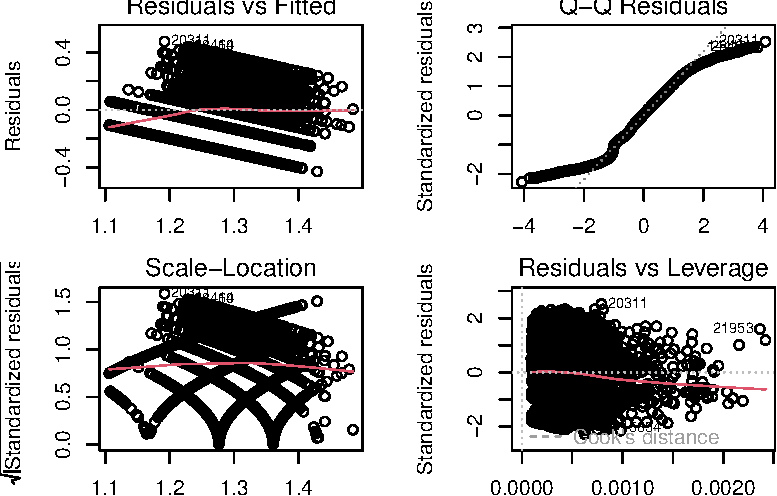
\includegraphics{project_report_files/figure-pdf/unnamed-chunk-37-1.pdf}

}

\end{figure}

\begin{Shaded}
\begin{Highlighting}[]
\CommentTok{\# Variable importance plot}
\NormalTok{importance\_matrix }\OtherTok{\textless{}{-}} \FunctionTok{xgb.importance}\NormalTok{(}\AttributeTok{feature\_names =} \FunctionTok{colnames}\NormalTok{(train\_matrix), }\AttributeTok{model =}\NormalTok{ xgb\_model)}
\FunctionTok{xgb.plot.importance}\NormalTok{(importance\_matrix)}
\end{Highlighting}
\end{Shaded}

\begin{figure}[H]

{\centering 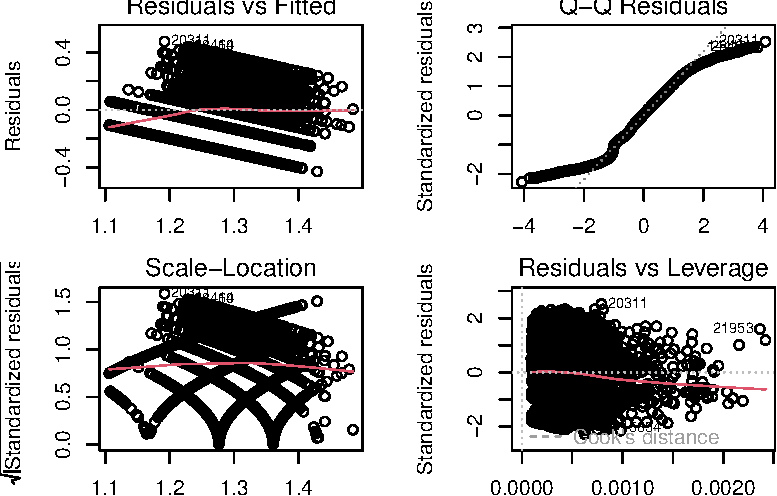
\includegraphics{project_report_files/figure-pdf/unnamed-chunk-38-1.pdf}

}

\end{figure}

\begin{Shaded}
\begin{Highlighting}[]
\CommentTok{\# Mean Absolute Error}
\NormalTok{mae }\OtherTok{\textless{}{-}} \FunctionTok{mean}\NormalTok{(}\FunctionTok{abs}\NormalTok{(true\_values }\SpecialCharTok{{-}}\NormalTok{ xgb\_predictions))}
\FunctionTok{print}\NormalTok{(}\FunctionTok{paste}\NormalTok{(}\StringTok{"MAE:"}\NormalTok{, mae))}
\end{Highlighting}
\end{Shaded}

\begin{verbatim}
[1] "MAE: 1.90328994001195"
\end{verbatim}

\begin{Shaded}
\begin{Highlighting}[]
\CommentTok{\# Residuals plot}
\NormalTok{residuals }\OtherTok{\textless{}{-}}\NormalTok{ true\_values }\SpecialCharTok{{-}}\NormalTok{ xgb\_predictions}
\FunctionTok{plot}\NormalTok{(residuals, }\AttributeTok{type =} \StringTok{"l"}\NormalTok{, }\AttributeTok{main =} \StringTok{"Residuals Plot"}\NormalTok{, }\AttributeTok{xlab =} \StringTok{"Index"}\NormalTok{, }\AttributeTok{ylab =} \StringTok{"Residual"}\NormalTok{)}
\FunctionTok{abline}\NormalTok{(}\AttributeTok{h =} \DecValTok{0}\NormalTok{, }\AttributeTok{col =} \StringTok{"red"}\NormalTok{)}
\end{Highlighting}
\end{Shaded}

\begin{figure}[H]

{\centering \includegraphics{project_report_files/figure-pdf/unnamed-chunk-40-1.pdf}

}

\end{figure}

\hypertarget{references}{%
\section*{References}\label{references}}
\addcontentsline{toc}{section}{References}

\hypertarget{bibliography-styles}{%
\section{Bibliography styles}\label{bibliography-styles}}

Here are two sample references: \citet{Feynman1963118}
\citet{Dirac1953888}.

By default, natbib will be used with the \texttt{authoryear} style, set
in \texttt{classoption} variable in YAML. You can sets extra options
with \texttt{natbiboptions} variable in YAML header. Example

\begin{verbatim}
natbiboptions: longnamesfirst,angle,semicolon
\end{verbatim}

There are various more specific bibliography styles available at
\url{https://support.stmdocs.in/wiki/index.php?title=Model-wise_bibliographic_style_files}.
To use one of these, add it in the header using, for example,
\texttt{biblio-style:\ model1-num-names}.

\hypertarget{using-csl}{%
\subsection{Using CSL}\label{using-csl}}

If \texttt{cite-method} is set to \texttt{citeproc} in
\texttt{elsevier\_article()}, then pandoc is used for citations instead
of \texttt{natbib}. In this case, the \texttt{csl} option is used to
format the references. By default, this template will provide an
appropriate style, but alternative \texttt{csl} files are available from
\url{https://www.zotero.org/styles?q=elsevier}. These can be downloaded
and stored locally, or the url can be used as in the example header.


  \bibliography{bibliography.bib}


\end{document}
